\chapter{Photonics systems}
\section{Optical amplification}
\subsection{Introduction}
Il est nécessaire d'amplifier pour limiter les pertes dues à la propagation. Il y a différentes
applications 
\begin{itemize}
\item[$\bullet$] Si l'amplification est de trop haute puissance, on va rencontrer des effets 
non-linéaires. Si elle est trop basse, on ne captera rien. Dans les long-haul systems, on place
des \textbf{in-line amplifiers} tous les 50-80km.
\item[$\bullet$] \textbf{Power boosters} : juste après la source, pour atteindre 100-200km.
\item[$\bullet$] \textbf{Optical preamplifier} : juste avant le récepteur.
\item[$\bullet$] Pour compenser les pertes de distribution.
\end{itemize}

\subsection{General concepts}
La plupart des amplificateurs se basent sur le principe de l'émission stimulée. Comme pour les laser, 
on retrouve un milieu à gain dans lequel la lumière est amplifiée durant son passage. Le pompage peut
être électrique (semiconducteurs), optique (fibré) ou aussi de type Raman où il n'y a pas d'inversion de
population.

\subsubsection{Gain and bandwidth (two-level system)}
	\begin{wrapfigure}[8]{l}{3.6cm}
	\vspace{-5mm}
	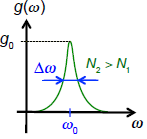
\includegraphics[scale=0.8]{ch6/image1}
	\captionof{figure}{ }
	\end{wrapfigure}
Lorsque le signal d'entrée est suffisamment faible, le gain $g(\omega)$ (m$^{-1}$) est indépendant 
de la puissance. C'est le régime non saturé. Dans un système à deux niveaux, la largeur naturelle de
gain est donnée par n
\begin{equation}
g(\omega ) = \frac{{{g_0}}}{{1 + 4{{(\omega  - {\omega _0})}^2}T_2^2}}
\end{equation}
Dans le régime d'amplification, celle-ci est décrite par une loi de Beer-Lambert avec une "absorption
négative"
\begin{equation}
\frac{{{\rm{d}}P(z)}}{{{\rm{d}}z}} =  + g(\omega )P
\end{equation}
Le profil de gain a une forme Lorentzienne. Il possède un maximum à la fréquence de la transition 
atomique $\omega_0$. On défini la largeur de gain (FWHM) comme $\Delta\omega_g = 1/T_2$ où $T_2$
est le temps de relaxation du dipôle. En communication, on préfère éviter d'avoir un gain très 
piqué, sans quoi seulement quelques canaux seraient amplifiés\footnote{Par chance, les amplificateurs
Erbium couvrent toute la bande $C$!}.

\newpage
	\begin{wrapfigure}[11]{r}{5cm}
%	\vspace{-5mm}
	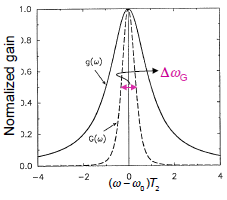
\includegraphics[scale=0.8]{ch6/image2}
	\captionof{figure}{ }
	\end{wrapfigure}
Souvent, on défini un amplificateur par sa la largeur de bande d'amplification qui est reliée à la
FWHM du gain d'amplification (facteur d'amplification) $G$ (et non pas via $g(\omega)$)
\begin{equation}
G = \frac{{{P_{out}}}}{{{P_{in}}}} = {{\mathop{\rm e}\nolimits} ^{g(\omega )L}}
\end{equation}
La FWHM est donnée par
\begin{equation}
\Delta {\omega _G} = \Delta {\omega _g}{\left[ {\ln (2)/\ln ({G_0}/2)} \right]^{1/2}}
\end{equation}
Celle-ci décroit avec $G_0=\exp(g_0L)$. On remarque que le \textbf{gain d'amplification} $G(\omega)$
décroit plus rapidement que le \textbf{gain optique} $g(\omega)$.

\subsubsection{Gain saturation}
La valeur maximale de $P_{out}$ est limitée\footnote{Souvent limité par la source externe.}. Pour
des signaux "importants", le gain optique peut dépendre de la puissance impliquant une diminution 
de $G$ lorsque la puissance du signal augmente (car $g(\omega)$ devient de plus en plus petit lorsque
la puissance augmente, c'est la saturation du gain). Le gain devient
\begin{equation}
g(\omega ) = \frac{{{g_0}}}{{1 + 4{{(\omega  - {\omega _0})}^2}T_2^2 + P/{P_{sat}}}}
\end{equation}
où $P_{sat}$ est la puissance de saturation, qui apparaissait naturellement en résolvant les 
équations de Maxwell-Bloch. Lorsque $P<P_{sat}$ le gain est celui à petit signal. Cependant lorsque
$P\approx P_{sat}$, $g$ devient plus petit que le gain à petit signal $g_0$.\\

Supposons que nous sommes à la résonance ($\omega=\omega_0$, gain maximum)
\begin{equation}
\frac{{{\rm{d}}P(z)}}{{{\rm{d}}z}} =  + gP = \frac{{{g_0}}}{{1 + P(z)/{P_{sat}}}}P(z)
\end{equation}
En intégrant l'ED
\begin{equation}
\int\limits_{{P_{in}}}^{{P_{out}}} {(\frac{1}{P} + \frac{1}{{{P_{sat}}}}){\rm{d}}P}  = \int\limits_0^L {{g_0}{\rm{d}}z} \qquad\Rightarrow\qquad
G = {G_0}\exp \left[ { - \frac{{G - 1}}{G}\frac{{{P_{out}}}}{{{P_{sat}}}}} \right]
\end{equation}
Il s'agit d'une relation implicite entre le facteur de gain actuel $G$ et la valeur de $G_0$ (soit
une relation implicite avec $P_{out}/P_{in}$). Cette relation montre que $G$ diminue avec $P_{out}$ et
que $G\ll G_0$ lorsque $P_{out}\to P_{sat}$.\\

Par définition, la \textbf{puissance de sortie à saturation} est la puissance de sortie tel que 
$G$ diminue de 3dB par rapport à la valeur non saturée $G_0$
\begin{equation}
G(P_{out}^s) = \frac{{{G_0}}}{2}\qquad\Rightarrow\qquad
P_{out}^s = {P_{sat}}\frac{{{G_0}\ln (2)}}{{{G_0} - 2}}
\end{equation}
Il s'agit d'un paramètre important pour caractériser les amplificateurs. Celui-ci est inférieur à 
$P_{sat}$ et indépendant de $G_0$ pour de grandes valeurs de ce-dernier.


\subsubsection{Amplifier noise}
Tous les amplificateurs dégradent le \textit{signal-to-noise ration} (SNR) (aussi bien optique que
électronique). Cette dégradation vient de l'émission spontanée dans les amplificateurs, qui ajoute
du bruit dans le signal amplifié. On quantifie la dégradation du SND avec le \textit{noise figure of
the amplifier} $F_n$
\begin{equation}
{F_n} = \frac{{{{(SN{R_e})}_{in}}}}{{{{(SN{R_e})}_{out}}}}
\end{equation}
où $SNR_e$ est le SNR électrique\footnote{Car au final, c'est ce que l'on va détecter.} (sans bruit)
mesuré avec un photo-détecteur idéal (limité par le shot-noise et$\eta = 1$).\\

Soit un signal d'entrée électrique, nous avons
\begin{equation}
{(SN{R_e})_{in}} = \frac{{{I_p}^2}}{{\sigma _S^2}} = \frac{{{{(R{P_{in}})}^2}}}{{2qR{P_{in}}\Delta f}} 
= \frac{{{P_{in}}}}{{2h\nu \Delta f}}
\end{equation}
La première égalité s'écrit sous l'hypothèse que le signal d'entrée est sans bruit ($I_{dark}=0$) 
et que le récepteur est idéal  : le bruit au récepteur est dominé par le shot-noise\footnote{$(SNR_e) = \frac{I_p^2}{\sigma^2}$ où $\sigma=\sigma_S$, le bruit thermique étant négligeable devant le shotnoise
.}. La seconde égalité vient du photo-détecteur idéal ($\eta=1\to R = q/h\nu$).\\

Pour le signal de sortie, c'est plus compliqué : il faut avoir un modèle du bruit et savoir comment il va jouer sur les fluctuations du courant\footnote{Soit quantifier l'impact de l'émission 
spontanée sur le SNR.}. Le calcul sera fait dans le contexte des amplificateurs dopés à l'erbium.\\

En plus de causer des variations d'amplitudes, l'émission spontanée cause également des fluctuations
de la phase du signal amplifié\footnote{Même si ces fluctuations sont petites, sur plus de 1000km on 
voit la différence. }. La phase initial $\omega_0$ est shiftée de $\delta\omega$ (comme si
la fréquence de la porteuse) de façon aléatoire. Comme la vitesse de groupe dépend de la 
fréquence
\begin{equation}
{v_g} = 1/[\beta '({\omega _0})\; + \delta \omega \beta ({\omega _0})\;]
\end{equation}
\begin{center}
	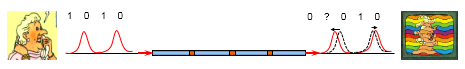
\includegraphics[scale=0.8]{ch6/image3}
	\captionof{figure}{La vitesse à laquelle les impulsions de signal se propagent est affectée de
	 manière aléatoire après chaque amplificateur.}
\end{center}
Le temps de vol de chaque impulsion est légèrement différent à cause de la dispersion de la vitesse
de groupe. Le bruit optique ou encore \textbf{ASE} (amplified spontaneous emission) est ainsi 
responsable de fluctuations aléatoires dans le temps d'arrivée de chaque bit dans son slot. On parle
de \textit{Gordon-Haus jiter}, qui impose une limitation fondamentale pour les systèmes long-haul.

\newpage
\subsection{Erbium-doped fiber amplifiers}
	\begin{wrapfigure}[14]{r}{10.5cm}
%	\vspace{-5mm}
	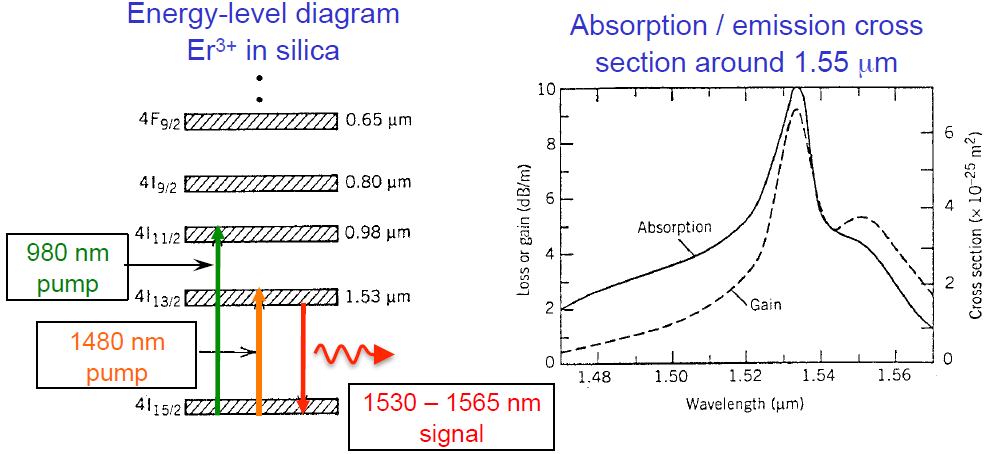
\includegraphics[scale=0.4]{ch6/image4}
	\captionof{figure}{Le passage d'une courbe à l'autre dépend de $N_i$}
	\label{fig:Er}
	\end{wrapfigure}
L'amplificateur optique le plus commun dans les systèmes de télécommunication est l'\textit{
erbium-doped fiber amplifier} \textbf{EDFA} (pour la bande $C$, 1530-1565nm). Le cœur d'une telle 
fibre est dopée avec des ions d'erbium (le verre de la fibre joue le rôle du milieu hôte). Ci-contre,
les niveaux d'énergie des ions erbium. Chaque niveau d'énergie est divisé en sous-niveau : on peut
représenter les niveaux d'énergies par des bandes\footnote{Nature amorphe du verre rend la séparation
des niveaux différent pour chaque ion}. Ainsi, on peut pomper aux alentours de 980nm ou 1480nm. En 
pompant à 980nm, on crée de l'absorption vers la troisième bande qui se désexcite rapidement vers
la seconde bande puis vers le fondamental par émission radiative (spontanée ou stimulée) dans la gamme
1530-1565nm. Sur le schéma de droite est représenté la section efficace d'absorption et la section
efficace de gain. On voit que le pompage à 1480nm est possible car la section efficace d'absorption y
est plus grande que la section efficace de gain.\\

L'émission stimulée et l'absorption (des ions d'erbium) sont caractérisés par les \textbf{sections
efficaces} $\sigma^e$ et $\sigma^a$
\begin{equation}
\frac{{\partial P}}{{\partial z}} = (\sigma _{}^e{N_2} - \sigma _{}^a{N_1})P
\end{equation}
\begin{itemize}
\item[$\bullet$] Si $N_2\gg N_1\to g(\omega) = \sigma^eN_2$
\item[$\bullet$] Si $N_2\ll N_1\to \alpha(\omega) = \sigma^aN_1$
\end{itemize}\ 


	\begin{wrapfigure}[8]{r}{6.5cm}
	\vspace{-5mm}
	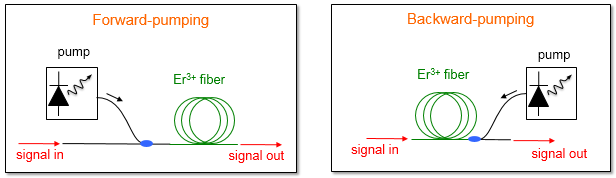
\includegraphics[scale=0.4]{ch6/image5}
	\captionof{figure}{ }
	\end{wrapfigure}
Pour l'EDFA, le pompage optique est efficace pour 980nm ou 1480nm (laser SC). L'avantage de l'EDFA est
qu'il possède une large bande de gain (35nm) pouvant amplifier simultanément plusieurs signaux dans
la bande C (plusieurs canaux de WDM dans la bande $C$ en même temps).\\

Deux configurations de pompage sont possibles : "avant" ou "après" la fibre. Pour se faire, on utilise
un WDM 980/1550. En terme de performance, il n'y a pas de différence \textbf{mais} le \textit{noise
figure} $F_n$ peut différer. Parfois, on fait les deux.\\

	\begin{wrapfigure}[6]{l}{6.5cm}
	\vspace{-7mm}
	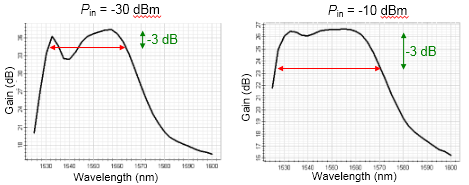
\includegraphics[scale=0.5]{ch6/image6}
	\captionof{figure}{ }
	\end{wrapfigure}
Nous avons vu que lorsque le signal devient grand, le gain d'amplification diminue par rapport au gain 
à petit signal(saturation). Ceci a pour conséquence que le gain d'amplification $G$ est 
"plus plat"\footnote{On le voit comment?} que la section efficace d'émission (dans le régime saturé
donc) et la bande passante de l'amplificateur est forcément plus grande que dans le régime insaturé. 
Ci-contre, le graphique de droite est plus proche de la saturation que celui de gauche. On constate 
effectivement un gain plus "plat" : on travaillera proche de la saturation.


\subsubsection{Simple two-level model of the EDFA}
Considérons que les deux populations atomiques $N_1$ et $N_2$, la puissance de pompe $P_p$ et du
signal $P_s$ sont gouvernées par les équations de bilan. Trois hypothèses
\begin{enumerate}
\item \textit{Interaction avec un système à deux niveaux}.\\
En réalité, il faut trois niveaux pour faire de l'amplification. Cependant, sa durée de vie est courte
: il est presque vide.
\item \textit{L'ASE est négligée}.\\
On ne considère que l'absorption et l'émission stimulée. L'ASE est cependant bien possible, mais on ne
la prend pas en compte dans l'évolution de l'onde du signal. 
\item \textit{Le profil des modes et les variations de densité atomique transverses sont négligées.}\\
On ne considère qu'une seule dimension spatiale $z$, le long de la fibre. 
\end{enumerate}\ \\

\textsc{I. Équations de la densité atomique}\\
Sous les précédentes hypothèses, l'équation régissant la dynamique de l'état de population dans 
le niveau supérieur est
\begin{equation}
\frac{{\partial {N_2}}}{{\partial t}} = (\sigma _p^a{N_1} - \sigma _p^e{N_2}){\phi _p} + (\sigma _s^a{N_1} - \sigma _s^e{N_2}){\phi _s} - \frac{{{N_2}}}{{{T_1}}}\qquad(1)
\end{equation}
On retrouve l'absorption de la pompes et du signal par les ions dans l'état fondamental ainsi que
l'émission stimulée à la pompe et à la longueur d'onde du signal. Le dernier terme correspond à 
la désintégration spontanée de l'état excité (durée de vie $T_1$). On notera plus particulièrement
\begin{itemize}
\item[$\bullet$] $\sigma$, la section efficace (m$^{-2}$) d'absorption et d'émission à la longueur
d'onde de la pompe et du signal
\item[$\bullet$] ${\phi _{p,s}} = {P_{p,s}}/(S.h{\nu _{p,s}})$ le flux de photons (s$^{-1}$m$^{-2}$)
où $S$ est la section transversale du mode.
\item[$\bullet$] $T_1$ le temps de vie de la fluorescence (spontanée) ($T_1=10$ms pour l'EDFA).
\end{itemize}\ 

La relation suivante nous donne directement l'équation de bilan pour $N_1$
\begin{equation}
{N_1} + {N_2} = N \Rightarrow \frac{{\partial {N_1}}}{{\partial t}} =  - \frac{{\partial {N_2}}}
{{\partial t}}\qquad(2)
\end{equation}\ \\

\textsc{II. Équation pour les champs (puissance)}\\
L'évolution de la puissance du signal avec $z$ est donnée par
\begin{equation}
\frac{{\partial {P_s}}}{{\partial z}} = (\sigma _s^e{N_2} - \sigma _s^a{N_1}){P_s} - \alpha _s^f\;{P_s}\qquad(3)
\end{equation}
L'évolution du signal de pompe est lui donné par
\begin{equation}
s\frac{{\partial {P_p}}}{{\partial z}} = \;(\sigma _p^e{N_2} - \sigma _p^a{N_1}){P_p} - \alpha _p^f\;{P_s}\qquad(4)
\end{equation}
où $s=\pm1$ selon le sens du pompage. Nous allons faire l'hypothèse que la longueur de d'amplificateur
est petite (quelques dizaines de mètres) de sorte à considérer $\alpha_{p/s}^f\approx0$. On remarque
que ces deux équations ne sont que les équations de Beer-Lambert où le gain est explicité en fonction
des densités atomiques. Elles ne tiennent pas compte de l'émission spontanée, très faible (et de plus,
peu se retrouvent dans la fibre et dans le mode que l'on cherche à amplifier\footnote{Si le signal
est très petit, ce n'est plus le cas.}.\\

Faisons deux hypothèse supplémentaires
\begin{itemize}
\item[4.] \textit{La fibre est courte}.\\
On néglige ses pertes
\item[5.] \textit{Propagation d'un signal continu (de même pour la pompe) et équation stationnaire
($\partial N_2/\partial t=0$}.
\end{itemize}\ 

A partir de $(1)$, on peut extraire une expression de $N_2(z)$ fonction des densités atomiques et 
des flux de photons du signal et de la pompe
\begin{equation}
{N_2}(z) = {T_1}\left( {(\sigma _p^a{N_1} - \sigma _p^e{N_2}){\phi _p} + (\sigma _s^a{N_1} - \sigma _s^e{N_2}){\phi _s}} \right)
\end{equation}
En utilisant $(3)$ et $(4)$, la précédente relation devient
\begin{equation}
N_2(z)  =  - \frac{{s{T_1}}}{{Sh{\nu _p}}}\frac{{{\rm{d}}{P_p}}}{{{\rm{d}}z}} - \frac{{{T_1}}}{{Sh{\nu _s}}}\frac{{{\rm{d}}{P_s}}}{{{\rm{d}}z}}
\end{equation}
où $\phi_s= P_s/(Sh\nu_s)$. En combinant cette dernière équation avec à nouveau l'équation $(3)$, on
trouve une EDO1 qui peut être intégrée
\begin{equation}
\frac{{{\rm{d}}{P_s}}}{{{\rm{d}}z}} = [\sigma _s^e{N_2} - \sigma _s^a(N - {N_2})]{P_s}
= \left( { - s\frac{{{T_1}(\sigma _s^e + \sigma _s^a)}}{{Sh{\nu _p}}}\frac{{{\rm{d}}{P_p}}}{{{\rm{d}}z}} - \frac{{{T_1}(\sigma _s^e + \sigma _s^a)}}{{Sh{\nu _s}}}\frac{{{\rm{d}}{P_s}}}{{{\rm{d}}z}} - \sigma _s^aN} \right){P_s}
\end{equation}
Celle-ci nous donne l'évolution de la puissance du signal. On y trouve l'absorption de l'onde du 
signal $\alpha_s = \sigma_s^aN$. En considérant la saturation intrinsèque de la puissance du signal
($\nu_s\approx\nu_p=\nu$)
\begin{equation}
P_s^{IS} = \frac{{Sh\nu }}{{{T_1}(\sigma _s^e + \sigma _s^a)}}
\end{equation}
L'équation devient
\begin{equation}
\frac{{{\rm{d}}{P_s}}}{{{P_s}}} =  - \left( {\frac{1}{{P_s^{IS}}}(s\frac{{{\rm{d}}{P_p}}}{{{\rm{d}}z}} + \frac{{{\rm{d}}{P_s}}}{{{\rm{d}}z}}) + {\alpha _s}} \right){\rm{d}}z
\end{equation}
Celle-ci n'est modélisée que par deux paramètres : la puissance de saturation intrinsèque à la 
longueur d'onde du signal et la coefficient d'absorption\footnote{Celui-ci est relié à l'absorption
par les ions d'erbium lorsque ceux-ci se trouvent dans le fondamental. C'est donc l'absorption 
subie par le signal lorsqu'il n'y a pas de pompe, si le signal d'entrée est suffisamment faible.}. \\

Intégrons cette ED entre le début ($z=0$) et la fin ($z=L$) de l'amplificateur ($s=1$)
\begin{equation}
P_s^{out} = P_s^{in}{e^{ - {\alpha _s}L}}{e^{({P^{in}} - {P^{out}})/P_s^{IS}}}
\end{equation}
Il s'agit de l'expression de la puissance de sortie du signal en fonction de la puissance totale
d'entrée ${P^{in}} = P_p^{in} + P_s^{in}$ et de la puissance totale de sortie ${P^{out}} = P_p^{out}
+ P_s^{out}$. Par un raisonnement similaire, pour la pompe 
\begin{equation}
P_p^{out} = P_p^{in}{e^{ - {\alpha _p}L}}{e^{({P^{in}} - {P^{out}})/P_p^{IS}}}
\end{equation}
où ${\alpha _p} = \sigma _p^aN$ et $P_p^{IS} = \frac{{Sh\nu }}{{{T_1}(\sigma _p^e + \sigma _p^a)}}$.\\

La puissance totale de sortie s'obtient en sommant les deux contributions\\

\cadre{\begin{equation}
\sum {}  \Rightarrow P_{}^{out} = P_s^{in}{e^{ - {\alpha _s}L}}{e^{({P^{in}} - {P^{out}})/P_s^{IS}}} + P_p^{in}{e^{ - {\alpha _p}L}}{e^{({P^{in}} - {P^{out}})/P_p^{IS}}}
\end{equation}}\ \\

Il s'agit d'une équation transcendantale en $P^{out}$ (tout est connu, sauf lui). La résolution 
de cette équation donnera $P^{out}$ et donc $P^{out}_s$. Quelques remarques avant d'aborder la 
résolution numérique
\begin{itemize}
\item[$\bullet$] Il y a seulement deux paramètres dépendant de la longueur : l'atténuation $\alpha$ et
la puissance de saturation intrinsèque $P^{IS}$
\item[$\bullet$] Le gain d'amplification et les caractéristiques de saturation sont indépendantes
de la configuration de pompage (soit le signe de $s$)
\item[$\bullet$] Le modèle peut être généralisé à $N$ faisceaux, mais l'équation sera toujours
transcendantale. 
\item[$\bullet$] Le modèle est toujours valable quand la puissance de signal d'entrée domine la 
puissance d'entrée du bruit.
\end{itemize}\ 

	\begin{wrapfigure}[12]{l}{6.5cm}
	\vspace{-3mm}
	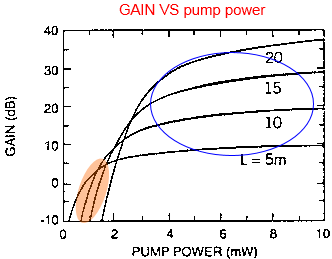
\includegraphics[scale=0.65]{ch6/image7}
	\captionof{figure}{ }
	\end{wrapfigure}
Ci-contre, la résolution numérique d'un amplificateur donné (longueur fixée). Pour une petite 
puissance, le gain est négatif (orange) et celui-ci sature lorsque la puissance de pompage devient grande (rond bleu). En effet, à petite puissance l'énergie est totalement absorbée par l'amplificateur
: les ions Er restent dans l'état fondamental et absorbent une partie du signal. Pour une grande
puissance de pompe, tous les atomes sont dans un états excité et le gain ne peut plus augmenter (le
milieu devient transparent, avoir une pompe plus puissante ne sert à rien). On remarque également que,
pour une puissance d'entrée importante, le facteur d'amplification augmente avec la longueur de
l'amplificateur\footnote{Pour des petites puissances de pompe, l'augmentation du gain est
exponentielle}.  \\

	\begin{wrapfigure}[9]{r}{4cm}
	\vspace{-5mm}
	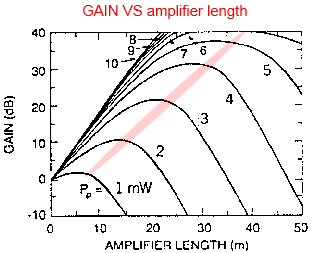
\includegraphics[scale=0.5]{ch6/image8}
	\captionof{figure}{ }
	\end{wrapfigure}
Ci-contre est représenté l'évolution du gain en fonction de la longueur de l'amplificateur, pour
différente puissances de pompes. On voit que pour une longueur donnée, il existe une longueur qui
maximise le gain : au delà de cette longueur, le gain diminue car le signal est absorbé par les
ions non excités. La longueur optimale $L_{opt}$ \textbf{dépend} de la puissance de pompe, on ne peut
pas les choisir indépendamment. \\

	\begin{wrapfigure}[8]{l}{7cm}
	\vspace{-11mm}
	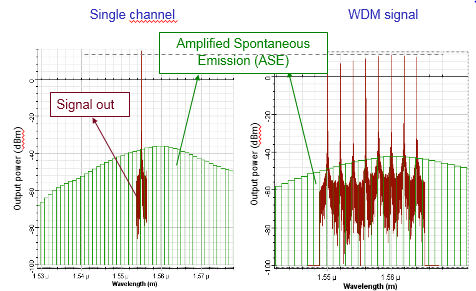
\includegraphics[scale=0.5]{ch6/image9}
	\captionof{figure}{ }
	\end{wrapfigure}
Considérons maintenant la simulation numérique du signal d'amplification en présence d'ASE : à la 
fois le signal et l'émission spontanée sont amplifiés. A gauche, un seul canal est utilisé et 
plusieurs sont utilisés à droite. On remarque que l'amplification est plus importante lorsqu'un seul
signal est amplifié. Dans un système à WDM, la puissance moyenne dans un canal à la sortie de 
l'amplificateur dépend de la présence et du nombre de signaux à d'autres longueurs d'onde : cause
des fluctuations du signal de puissance au récepteur\footnote{D'où l'importance de contrôler le gain
automatiquement dans chaque canal du bloc récepteur!}. Les plus observateurs remarqueront que l'ASE
est également réduit lorsque plusieurs canaux sont utilisés\footnote{On verra en effet que l'ASE dépend linéairement du facteur d'amplification.}. \\

Quelques discussions sur ces résultats
\begin{itemize}
\item[$\bullet$] Il y a toujours du bruit à cause de l'ASE, mais la saturation causée par 
l'amplification réduit son niveau.
\item[$\bullet$] L'effet de "saturation de gain croisé" est une source de cross-talk entre les
canaux commun à tous les amplificateurs optiques.
\item[$\bullet$] La non-uniformité du gain est une limitation de l'EDFA.
\end{itemize}


\subsubsection{Amplification of pulses in EDFA}
Jusqu'ici nous nous sommes intéressés à l'amplification de signaux continus, mais qu'en est-il des
impulsions (important pour le codage d'informations) ? Ce n'est pas évident car la réponse 
dépend de l'énergie de l'impulsion. Pour avoir la réponse à la question, nous allons résoudre les 
équations de bilan en prenant en compte le profil du pulse. Heureusement, lorsque la \textbf{durée du
pulse} est \textbf{plus courte} que le temps de fluorescence $T_1$, le système est facilement
résolvable avec une pompe continue et un signal pulsé. \\

Partons de l'équation de l'équation de bilan $(1)$ décrivant l'évolution de $N_2$
\begin{equation}
\frac{{\partial {N_2}}}{{\partial t}} = (\sigma _p^a{N_1}){\phi _p} + \sigma _s^{}({N_1} - {N_2}){\phi 
_s} - \frac{{{N_2}}}{{{T_1}}}
\end{equation}
où on suppose $\sigma_p^e\approx0$ (émission à la longueur d'onde de la pompe négligeable
\footnote{C'est-à-dire que le taux d'émission stimulée à cette longueur d'onde est négligeable par  
taux de décroissance du niveau $3\to2$ des ions d'Er. Cette dernière est rapide et la population 
atomique est soit dans le premier état excité, soit dans le fondamental, c'est à dire $N=N_1+N_2$.}) 
et que les sections efficaces d'émission et d'absorption sont à peu près les même à la longueur d'onde
du signal $\sigma _s^e \approx \sigma _s^a = \sigma _s^{}$. Ceci se justifie avec la \autoref{fig:Er}.

Par définition du gain optique, en introduisant l'inversion de population $\mathcal{D}$ on peut 
ré-écrire $N_1$ et $N_2$
\begin{equation}
g = \sigma _s^{}({N_2} - {N_1}) = \sigma _s^{}{\cal D}
\end{equation}
où ${N_1} = (N - {\cal D})/2$ et ${N_2} = (N + {\cal D})/2$. On trouve alors la variation du gain
à une position donnée $z$ dans l'amplificateur en fonction du temps
\begin{equation}
\frac{{\partial g(z,t)}}{{\partial t}} =  - g(\sigma _p^a{\phi _p} + \frac{1}{{{T_1}}}) + N\sigma
_s^{}(\sigma _p^a{\phi _p} - \frac{1}{{{T_1}}}) - 2g\sigma _s^{}{\phi _s}
\end{equation}\ \\

S'il n'y a pas de signal d'entrée ($\phi_s=0$), on retrouve le gain à petit signal $g_0$ en étudiant
le cas stationnaire (logique, car pas de signal d'entrée c'est un "petit" signal)
\begin{equation}
{g_0} = N\sigma _s^{}({T_1}\sigma _p^a{\phi _p} - 1)/({T_1}\sigma _p^a{\phi _p} + 1)
\end{equation}
où $g_0>0$ lorsque $\sigma _p^a{\phi _p}{T_1} > 1$. Il s'agit d'une condition sur le signal de 
pompe pour avoir inversion de la population. \\

On peut donc ré-écrire l'équation différentielle pour $g$ qui dépend maintenant de $g_0$
\begin{equation}
\frac{{\partial g(z,t)}}{{\partial t}} = ({g_0} - g)(\sigma _p^a{\phi _p} + \frac{1}{{{T_1}}}) - 2g
\sigma _s^{}{\phi _s}(z,t)
\label{eq:ASimplif}
\end{equation}
Écrivons le flux de photons du signal en fonction de la puissance d'entrée
\begin{equation}
{\phi _s}(z,t) = \frac{{{P_s}(z,t)}}{{Sh{\nu _s}}}
\end{equation}
où $S$ est la surface effective du faisceau, qui prend en compte le profil du mode exact. Introduisons
également la saturation en énergie intrinsèque du milieu à la longueur d'onde du signal
\begin{equation}
E_s^{IS} = \frac{{Sh{\nu _s}}}{{2{\sigma _s}}} = P_s^{IS}{T_1}
\end{equation}
Cette énergie joue le même rôle que la puissance de saturation, mais pour l'amplification de pulse et
non pas d'un signal continu\footnote{Lorsque l'énergie du pulse est éloigné de cette valeur, le gain
est non-saturé mais le gain est réduit lorsqu'on s'approche de cette valeur. Elle vaut à peu près
10$\mu$J pour l'EDFA (valeur énorme).}. \\

Nous allons essayer de simplifier \eqref{eq:ASimplif} en limitant l'équation à l'utilisation en 
télécommunications. En NRZ, 1Gbits/s donne un temps bit de l'ordre de la ns (durée de l'impulsion).
C'est beaucoup plus court que la durée de vie de la fluorescence $T_1\approx 10$ms et que le 
temps caractéristique de pompage $(\sigma_p^a\phi_p)^{-1}$. Le premier terme ($\propto (g-g_0)$) 
peut alors être négligé durant l'amplification du pulse
\begin{equation}
\frac{{\partial g(z,t)}}{{\partial t}} =  - g{P_s}(z,t)/E_s^{IS}
\end{equation}
Cette équation s'intègre facilement
\begin{equation}
\int_{{g_0}}^{g(t)} {\frac{{dg}}{g}}  =  - \int_{ - \infty }^t {{P_s}(\tau )/E_s^{IS}d\tau } 
\end{equation}
Ce qui donne
\begin{equation}
g(z,t) = {g_0}(z)\exp ( - \int_{ - \infty }^t {{P_s}(z,\tau )/E_s^{IS}d\tau } )
\end{equation}
Tant que l'énergie de l'impulsion du signal est inférieure à l'énergie de saturation, le gain n'est
pas affecté par l'amplification du pulse et il reste égal à $g_0$. L'énergie du pulse étant donnée par
\begin{equation}
{E_s}(z) = \int_{ - \infty }^{ + \infty } {{P_s}(t,z)dt}  <  < E_s^{IS}
\end{equation}
Celle-ci vaut à peu près $P.\Delta t = 1ns.1mW\approx pJ$ et donc l'exponentielle fait donc à peu près 1. Si le  gain ne varie pas, c'est parce que l'énergie transférée au pulse est négligeable par rapport
à  l'énergie "disponible" dans le milieu atomique. En conclusion, en télécommunication, le gain
peut être supposé constant et il ne dépend pas du modèle exact de l'impulsion. \\

\cadre{\begin{equation}
g(z,t) = {g_0}(z)
\end{equation}
Le gain ne varie pas de pulse à pulse et la saturation du gain est gouvernée par la 
\textbf{moyenne} du signal et pas la puissance de pic d'une impulsion.}

\newpage
\subsubsection{Amplifier noise in EDFA and the noise figure $F_n$}
	\begin{wrapfigure}[8]{l}{8.5cm}
	\vspace{-5mm}
	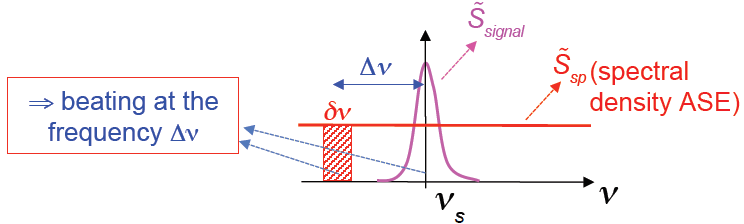
\includegraphics[scale=0.4]{ch6/image10}
	\captionof{figure}{ }
	\end{wrapfigure}
Dans l'EDFA, l'ASE ajoute du bruit au signal amplifié causant une dégradation (limité par le 
shot-noise, inévitable)  du $SNR_e$. Cette dégradation est quantifiée par la \textit{noise figure}
$F_n$ 
\begin{equation}
{F_n} = \frac{{{{(SN{R_e})}_{in}}}}{{{{(SN{R_e})}_{out}}}}
\end{equation}
Cette ASE va causer une fluctuation de la puissance du signal optique à case d'un battement entre
le signal à une longueur d'onde et l'ASE à une autre longueur d'onde.  Le battement entre deux 
bandes spectrales différentes dans l'ASE donne aussi lieu à des fluctuations de puissance. Il 
est donc nécessaire de calculer la densité spectrale de l'ASE!\\

\textsc{1. Spectral density of the ASE?}\\
Le but ici est de donner le nombre de photons à la sortie d'un amplificateur connaissant le nombre
de photons à son entrée, en tenant compte de l'émission spontanée à la longueur d'onde de travail. 
Faisons deux hypothèses
\begin{enumerate}
\item Le profil du monde et la densité atomique transverse sont négligés.
\item Système atomique à deux niveaux avec une densité spectrale de radiation\footnote{Densité d'énergie par
unité de volume et de fréquence.} $\rho_s(\nu)$ dans un guide d'onde monomode.
\end{enumerate}
Nous allons nous baser sur les taux d'absorption et d'émission
\begin{equation}
{R_{abs}} = \int {B\;f(\nu ){N_1}\;{\rho _s}d\nu },\qquad\qquad\qquad
{R_{stim}} = \int {B\;f(\nu ){N_2}\;{\rho _s}d\nu } 
\end{equation}
où $[N_j] = m^{-3}$ et où $f(\nu)$ est la \textit{lineshape function} qui inclus la dépendance de la 
fréquence des photons dan l'interaction lumière-matière. 


\begin{enumerate}
\item \textbf{Contribution cohérente}\\
Nous parlons ici de l'amplification d'une onde monochromatique. Il faut commencer par écrire la densité
spectrale de radiation
\begin{equation}
{\rho _s} = ({\phi _s}/{v_g})h{\nu _s}\delta (\nu  - {\nu _s})
\end{equation}
où $n_p$ est la densité d'énergie\footnote{Quantité d'énergie par unité de volume et de fréquence.}. On
peut la réécrire $n_p=\phi_p/v_g$, le flux de photons divisé par la vitesse de groupe. On en tire
\begin{equation}
\begin{array}{ll}
\DS\int_V \left(\phi_p/v_g\right) h\nu \int_\nu Bf(\nu)N_1 \delta(\nu-nu_s) d\nu dV &=\DS -\int \left(\phi_p/v_g\right) h\nu_s f(\nu_s)N_1 dV\vspace{2mm}\\
&=\DS -\int_V \left(\phi_p/v_g\right)dV h\nu_sBf(\nu_s)N_1\vspace{2mm}\\
&=\DS-Bf(\nu_s)h\nu_s N_p N_1
\end{array}
\end{equation}
car $\DS\int_V \left(\phi_p/v_g\right) dV = N_p$ avec $[N_p] = 1$ (\danger). Il s'agit du nombre d'absorption
par unité de temps et de volume. Sa variation est donnée par
\begin{equation}
\left.\dfrac{dN}{dt}\right|_{abs} = -\int R_{abs}\ dV
\end{equation}

En faisant de même pour l'émission spontanée, on peut en déduire
\begin{equation}
{\left. {\frac{d}{{dt}}{N_P}} \right|_{coh}} = \int {({R_{stim}} - {R_{abs}})} \;dV = Bf({\nu _s})h{\nu _s}({N_2} - {N_1}){N_P}
\end{equation}
Sachant que la vitesse de groupe est donnée par ${v_g} = c/{n_g} = {(\frac{{\partial \beta }}{{\partial \omega
 }})^{ - 1}}$, on en tire $\frac{d}{{dt}}{N_P} = {v_g}\frac{d}{{dz}}{N_P}$ de sorte à écrire
\begin{equation}
{\left. { \Rightarrow \frac{d}{{dz}}{N_P}} \right|_{coh}} = \sigma ({N_2} - {N_1}){N_P} = g{N_P}
\end{equation}
où l'on reconnaît la \textbf{section efficace "d'interaction"} $\sigma  = Bf({\nu _s})h{\nu _s}/{v_g}$. Le 
gain en $[m^{-1}]$ est donné par $\sigma(N_2-N_1)$.\\

\item \textbf{Distribution incohérente}\\
Plus dur, il faut prendre en compte l'émission spontanée. Comment écrire le taux d'émission spontané à 
$\nu_s$ dans le mode guidé ? Écrivons le taux \textit{total} d'émission spontané
\begin{equation}
{R_{sp}} = \int {A\;{N_2}f(\nu )d\nu }  = \int {\frac{{8\pi {\nu ^2}}}{{{c^3}}}h\nu \;B{N_2}f(\nu )d\nu } 
\end{equation}
où nous avons utilisé la définition du coefficient d'Einstein $A = \frac{{8\pi {\nu ^2}}}{{{c^3}}}h\nu B$.
Grâce à la densité spectrale de mode\footnote{Le nombre de modes par unité de volume et de fréquence}  
$(8\pi\nu^2/c^3)$, on calcule l'émission à toutes les fréquences. Or, ce qui nous intéresse, c'est uniquement
ce qui est émis dans le mode guidé : on veut pour un seule mode. On ne va plus considérer l'intégrale sur 
toute les fréquences et la remplacer par '1' pour n'avoir la contribution que d'un seule mode
\begin{equation}
{\left. {\frac{d}{{dz}}{N_p}} \right|_{incoh}} = (Bf({\nu _s})h{\nu _s}/{v_g}).1.{N_2} = \sigma {N_2}
\end{equation}
Il s'agit bien de l'émission spontanée à \textbf{un} mode, à \textbf{un} état de polarisation \textbf{et} à
$\nu_s$.\\

\item \textbf{En tenant les deux en compte}\\
En sommant les deux contributions
\begin{equation}
\frac{d}{{dz}}{N_p} = \sigma ({N_2} - {N_1})({N_p} + \frac{{{N_2}}}{{{N_2} - {N_1}}}) = g({N_p} + {n_{sp}})
\end{equation}
où ${n_{sp}} = {N_2}/({N_2} - {N_1})$ est le \textbf{facteur d'émission spontané}.
\end{enumerate}\ 

Maintenant que nous avons la contribution totale, il faut l'intégrer du début ($z=0$) à la fin de 
l'amplificateur ($z=L$)
\begin{equation}
\int\limits_{{N_p}(0)}^{{N_p}(L)} {\frac{{d{N_p}}}{{{N_p} + {n_{sp}}}} = \int\limits_0^L {gdz} }\qquad
\Rightarrow\qquad
 \Rightarrow {N_p}(L) = [{N_p}(0) + {n_{sp}}]{e^{gL}} - {n_{sp}}
\end{equation}
où $N_p(0)$ est le nombre de photons au début de l'amplificateur et $N_p(L)$ le nombre à la fin (ce qu'on 
cherche). On en tire, en se souvenant que $G=e^{gL}$\\

\cadre{\begin{equation}
{N_p}(L) = G{N_p}(0) + (G - 1){n_{sp}}
\end{equation}
où $(G-1)n_{sp}$ est une phase aléatoire responsable du signal de bruit. Celle-ci est bien amplifiée ($G-1$).}\ \\

La contribution de l'\textbf{émission spontanée} est équivalent à\textbf{ l'amplification de $n_p$ photons} 
(par mode) dans un amplificateur idéal avec un facteur d'amplification $G-1$.\\


Lorsqu'il n'y a pas de signal d'entrée ($N_p(0)=0$), $N_p(L)$ donne l'émission spontanée amplifiée (ASE) dans le
mode guidé et à la fréquence $\nu$. La \textbf{densité spectrale d'ASE} (dans un état de polarisation) à la
sortie de l'amplificateur est \textit{presque constante} (bruit blanc) et peut s'écrire\\

\cadre{\begin{equation}
{\tilde S_{ASE}} = (G - 1){n_{sp}}h\nu 
\end{equation}}\ \\

Remarques
\begin{itemize}
\item[$\bullet$] Le niveau d'ASE est plus bas en présence d'un signal grâce aux effets de saturation du 
gain ($G\ll G_0$ quand $P_{out} \approx P_s^{IS}$).
\item[$\bullet$] Lorsque la section efficace d'absorption est différente de celle d'émission, le facteur
d'émission spontané s'écrit
\begin{equation}
{n_{sp}} = \sigma _s^e{N_2}/(\sigma _s^e{N_2} - \sigma _s^a{N_1})
\end{equation}
\item[$\bullet$] Pour un amplificateur idéal $N_2\gg N_1$ (inversion de population complète), $n_{sp}\to1$.
Souvent, on fait dès lors l'hypothèse que le bruit rajoute un photon par mode.
\end{itemize}\ \\

\textsc{2. Contribution of the ASE to the output SNR$_e$ ?}\\
Les photons incohérents générés par l'émission spontanée causent des fluctuations de l'amplitude du signal
électrique à cause d'un \textbf{battement} entre les photons à différentes fréquences. Le photo-courant s'écrit
	\begin{equation}
I(t) + I_p+i_S(t)+i_{S-ASE}(t)+i_{ASE-ASE}(t)
\end{equation}

	\begin{wrapfigure}[9]{l}{6cm}
	\vspace{-8mm}
	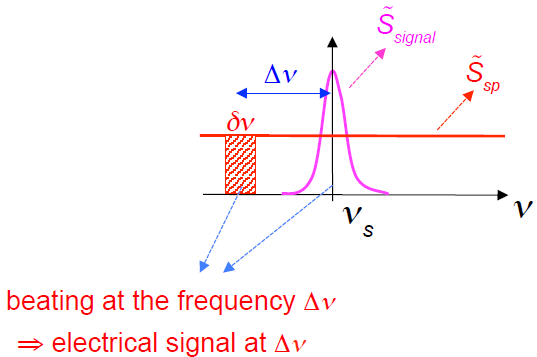
\includegraphics[scale=0.4]{ch6/image11}
	\captionof{figure}{ }
	\end{wrapfigure}
Même si l'amplitude de l'ASE est petite comparée à l'amplitude du signal, le battement $ASE-ASE$ peut être 
important car chaque paire de fréquence séparée de $\Delta\nu$ contribue aux fluctuations du courant à la
fréquence $\Delta\nu$. Pour minimiser la contribution du battement entre bandes spectrales séparée, on va
insérer un \textit{filtre optique} de bande passante $\Delta \nu_{opt}$ avant le récepteur\footnote{Limite le
nombre de paire possible.}. Ainsi, pour $G>10$ dB, la contribution principale du bruit vient de $i_{S-ASE}$.\\

Le photo-courant généré par le signal d'amplification étant $I = R.\sqrt G {E_{in}} + {E_{sp}}{^2}$, le \textbf{courant de bruit} résultant du battement \textit{signal-ASE} est donc
\begin{equation}
{i_{sig - ASE}}(t) = 2R\sqrt {G{P_{in}}} {E_{sp}}\cos [\Delta \phi (t)]
\end{equation}
où le terme $\cos(\dots)$ est responsable d'une phrase aléatoire variant rapidement.\\

On calcule la variance du signal de battement dans la bande passante du \textbf{récepteur} $\Delta f$ ainsi
que la moyenne sur les fluctuations comme nous avions fait pour le shot et thermal noise
\begin{equation}
\sigma _{sig - sp}^2 = 4{R^2}G{P_{in}}({\tilde S_{ASE}}2\Delta f).\frac{1}{2}
\end{equation}
On retrouve un $2\Delta f$ car le battement à $\Delta \nu$ peut provenir d'une bande décalée de $\Delta \nu$
ou décalée de $-\Delta \nu$. Encore une fois, il convient de regarder ici uniquement ce qui passe à travers
le filtre passe-bas. \\

On en déduit le SNR$_e$ de sortie
\begin{equation}
{(SNR)_{out}} = \frac{{I_p^2}}{{\sigma _s^2 + \sigma _{sig - sp}^2}} = \frac{{{{(RG{P_{in}})}^2}}}{{2qRG{P_{in}}\Delta f + 4{R^2}G{P_{in}}{{\tilde S}_{ASE}}\Delta f}}
\end{equation}
Comme $R=q/h\nu$ et $\tilde{S}_{ASE} =(G-1)n_{sp}h\nu$, on peut réécrire le SNR$_e$ à la sortie de 
l'amplificateur
\begin{equation}
{(SNR)_{out}} = \frac{{G{P_{in}}}}{{2h\nu \Delta f[1 + 2(G - 1){n_{sp}}]}}
\end{equation}
\ \\

\textsc{3. Noise figure $F_n$ of the amplifier?}\\
Maintenant que nous avons tous les éléments nécessaire en notre possession, nous pouvons calculer le $F_n$. 

\begin{description}
\item[Signal d'entrée]
\begin{equation}
{(SN{R_e})_{in}} = \frac{{{I_p}^2}}{{\sigma _S^2}} = \frac{{{{(R{P_{in}})}^2}}}{{2qR{P_{in}}\Delta f}} = \frac{{{P_{in}}}}{{2h\nu \Delta f}}
\end{equation}
où la première égalité suppose $I_{dark}=0$ et que nous sommes limités par le shot noise. La seconde 
égalité suppose que nous avons un photodétecteur idéal ($\eta=1$) : $R=q/h\nu$. \danger\ $\Delta f$ est
bien la bande passante du linear channel du \textbf{détecteur} !

\item[Signal de sortie]
\begin{equation}
{(SN{R_e})_{out}} = \frac{{I_p^2}}{{\sigma _s^2 + \sigma _{sig - sp}^2}} = \frac{{{{(RG{P_{in}})}^2}}}{{2qRG{P_{in}}\Delta f + 4{R^2}G{P_{in}}{{\tilde S}_{ASE}}\Delta f}} = \frac{{G{P_{in}}}}{{2h\nu \Delta f[1 + 2(G - 1){n_{sp}}]}}
\end{equation}
\end{description}

En effectuant le rapport des deux\\

\cadre{\begin{equation}
{F_n} = \frac{{{{(SNR)}_{in}}}}{{{{(SNR)}_{out}}}} = \frac{{{P_{in}}}}{{2h\nu \Delta f}}\frac{{2h\nu \Delta f[1 + 2(G - 1){n_{sp}}]}}{{G{P_{in}}}} = 2{n_{sp}}(1 - \frac{1}{G}) + \frac{1}{G} \approx 2{n_{sp}}
\end{equation}
La dernière "égalité" suppose que $G\gg1$.}\ \\

Cette expression est simplifiée car elle ne tient pas compte de la dépendance en $z$. Dans le cas du bruit le 
plus faible possible $n_{sp}=1$, on trouve $F_n=2$ soit une dégradation du SNR$_e$ de 3 dB. C'est le minimum
de bruit possible.\newpage

	\begin{wrapfigure}[14]{l}{9.5cm}
%	\vspace{-5mm}
	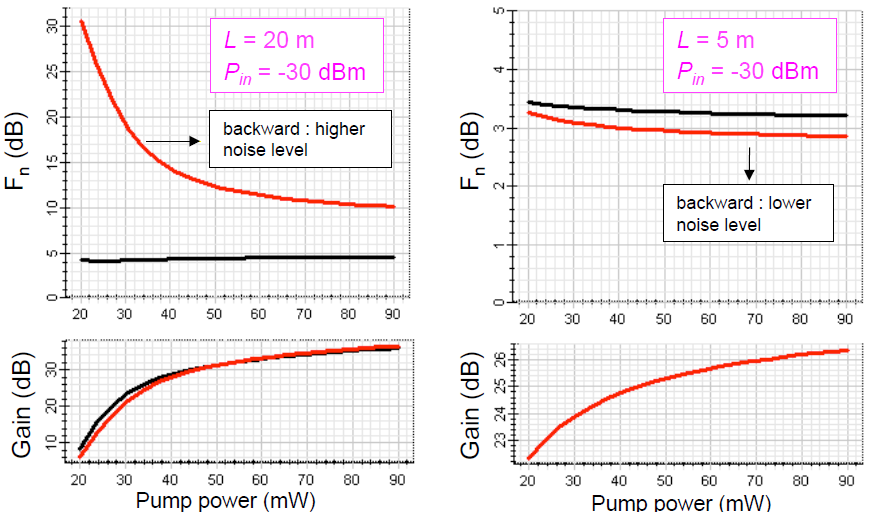
\includegraphics[scale=0.4]{ch6/image12}
	\captionof{figure}{ }
	\end{wrapfigure}
Regardons comment varie la figure de bruit. En noir nous avons le forward et en rouge le backward. On remarque 
que le gain est quasi identique pour les deux situations, mais pas le $F_n$. On remarque que la situation
\textit{backward} introduit un plus grand niveau de bruit, près de 30 dB pour une puissance de pompe peu 
élevée. En effet, si l'on pompe à la fin d'une longue fibre avec une faible puissance, nous aurons à l'avant
$N_1>N_2$ et à l'arrière $N_2>N_1$. En se propageant, le signal va d'abord diminuer par absorption puis il va
attaquer la région de gain avec un signal très faible, quasi nul. Il n'y a absolument pas d'effet de 
saturation du gain et le bruit d'ASE correspond au maximum que l'on peut avoir. Dans la situation inverse, on
augmentera exponentiellement le signal causant une saturation du gain, et donc, une diminution de l'ASE.

\subsubsection{Optical pre-amplification}
	\begin{wrapfigure}[7]{r}{9.5cm}
	\vspace{-9mm}
	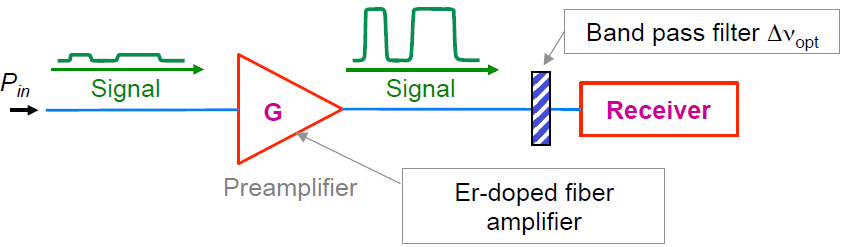
\includegraphics[scale=0.4]{ch6/image13}
	\captionof{figure}{ }
	\end{wrapfigure}
Une application de l'amplificateur optique est d'amplifier le signal juste avant le récepteur. Le but de ceci
est d'avoir une plus longue distance de propagation entre le transmetteur et le récepteur. Ce préamplificateur
va augmenter la puissance moyenne du signal qui atteint le récepteur mais aussi le bruit à cause de l'ASE. Dès
lors, \textit{la sensibilité du récepteur avec un préampli est-elle meilleure que le récepteur seul ?} Le 
SNR nous le dira.\\

\begin{itemize}
\item[$\bullet$] Si le récepteur est limité par le \textbf{shot noise}\\
\begin{equation}
{(SN{R_e})_{preamp}} = \frac{{SN{R_e}^{Shotnoise}}}{{{F_n}}}
\end{equation}
La dégradation est liée à $1/F_n$. Au mieux, on le diminue d'un facteur 2. Un préamplificateur optique n'aide pas
dans cette situation.

\item[$\bullet$] Cas général
\begin{equation}
{(SN{R_e})_{preamp}} = \frac{{I_p^2}}{{\sigma _s^2 + \sigma _{sig - ASE}^2 + \sigma _T^2}} = \frac{{{{(RG{P_{in}})}^2}}}{{2qRG{P_{in}}\Delta f + 4{R^2}G{P_{in}}{{\tilde S}_{ASE}}\Delta f + {F_{n,e}}(4{k_B}T/{R_L})\Delta f}}
\end{equation}
\begin{equation}
{(SN{R_e})_{PIN}} = \frac{{I_p^2}}{{\sigma _s^2 + \sigma _T^2}} = \frac{{{{(R{P_{in}})}^2}}}{{2qR{P_{in}}\Delta f + {F_{n,e}}(4{k_B}T/{R_L})\Delta f}}
\end{equation}
\end{itemize}
\newpage
Quand la sensibilité du récepteur est limitée par le bruit thermique, la pré-amplification augmente le SNR$_e$.
On peut montrer (\textit{slide 36}) que
\begin{equation}
{\bar P_{rec}} = 2{Q^2}\frac{{G - 1}}{G}{n_{sp}}h\nu \Delta f
\end{equation}
où $\Delta f$ est un filtre passe-bas dans le  récepteur ? \footnote{\textbf{A vérifier}}

\begin{center}
	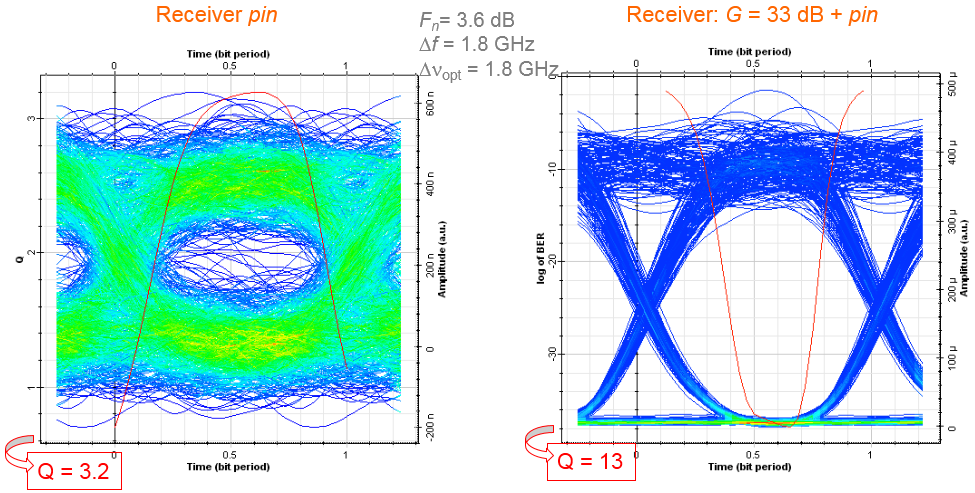
\includegraphics[scale=0.4]{ch6/image14}
	\captionof{figure}{ }
\end{center}


\subsubsection{Lumped amplification}
	\begin{wrapfigure}[7]{l}{7cm}
%	\vspace{-5mm}
	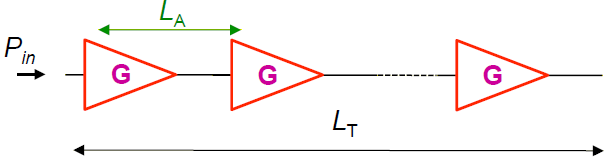
\includegraphics[scale=0.4]{ch6/image15}
	\captionof{figure}{ }
	\end{wrapfigure}
Les lignes de transmission \textit{long-haul} ont besoin de beaucoup d'amplificateurs pour compenser les
pertes fibrées. Soit $L_A$, la distance entre deux amplificateurs et $\exp(-\alpha L_A)$ les pertes entre
ces deux égales. Il faut au moins que la perte soit compensée par l'amplificateur de gain $G$
\begin{equation}
G = {e^{\alpha {L_A}}}
\end{equation}
Il ne faut pas oublier que chaque amplificateur ajoute de l'émission spontanée : l'ASE
augmente linéairement avec le nombre d'étages. L'ASE est préjudiciable pour deux raisons : elle dégrade 
le SNR et elle peut saturer l'amplificateur optique (diminution du gain).\\

L'ASE est augmentée\footnote{Linéairement, et pas amplifiée. A vérifier.} à chaque amplificateur mais 
est aussi atténuée entre deux étages. L'ajout net d'ASE de chaque amplificateur $\tilde{S}_{ASE}^1$ peut 
simplement être ajoutée
\begin{equation}
P_{ASE}^{tot} = 2{N_A}{\tilde S^1}_{ASE}\Delta {\nu _{opt}}
\end{equation}
La puissance totale prend en compte les deux polarisations (ASE non polarisée), le nombre total d'étages
$N_A=L_T/L_A$, la densité spectrale d'ASE et la bande passante du \textbf{filtre optique} dans le récepteur.
En explicitant
\begin{equation}
P_{ASE}^{tot} = 2{N_A}\Delta {\nu _{opt}}{n_{sp}}h\nu (G - 1)
\end{equation}
La puissance d'ASE augmente avec $N_A(G-1)$, elle peut devenir non-négligeable. Cependant, 
${N_A} = \frac{{{L_T}}}{{{L_A}}} = \frac{{\alpha {L_T}}}{{\ln (G)}}$. On peut réécrire cette expression
en fonction de $G$
\begin{equation}
P_{ASE}^{tot} = 2{n_{sp}}h\nu {L_T}\alpha \Delta {\nu _{opt}}(G - 1)/\ln (G)
\end{equation}
L'augmentation de la puissance de l'ASE est proportionnelle à $(G - 1)/\ln (G)$ : plus $G$ est petit à chaque
étage, moins l'ASE est important. De plus, plus $L_A$ est petit, plus la puissance d'ASE diminue. L'idéal est 
donc d'avoir un maximum d'étage avec le plus petit gain sur chacun, mais ça coûte cher. \\

Il y a un compromis entre le nombre d'amplificateurs et la dégradation du SNR$_o$. Ce dernier est défini par
\begin{equation}
SN{R_o} = \frac{{{P_s}}}{{P_{ASE}^{tot}}} = \frac{{{P_{in}}}}{{P_{ASE}^{tot}}} = \frac{{{P_{in}}\ln (G)}}{{2{n_{sp}}h\nu {L_T}\alpha \Delta {\nu _{opt}}(G - 1)}}
\end{equation}
En considérant ces deux expressions
\begin{equation}
SN{R_o} = \frac{{{P_s}}}{{P_{ASE}^{tot}}} = \frac{{{P_s}}}{{2{{\tilde S}_{ASE}}\Delta {\nu _{opt}}}},\qquad\qquad
Q \approx \frac{{{I_1}}}{{\sigma _{sig - ASE}^{}}} = \frac{{R{P_s}}}{{\sqrt {4{R^2}{P_s}{{\tilde S}_{ASE}}\Delta f} 
}}
\end{equation}
On peut mettre en évidence un lien entre le SNR$_o$ et le facteur de qualité $Q$
\begin{equation}
 \Rightarrow \;Q = \sqrt {SN{R_o}\;M/2} 
\end{equation}
où $M = \Delta {\nu _{opt}}/\Delta f$. Comme nous ne considérons ici que le signal de battement $ASE-ASE$
\begin{equation}
Q = \frac{{SN{R_o}\sqrt M }}{{\sqrt {2SN{R_o} + 1}  + 1}}
\end{equation}
L'expression devient
\begin{equation}
SN{R_o} = \frac{{2{Q^2}}}{M} + \frac{{2Q}}{{\sqrt M }} = \frac{{{P_s}}}{{2{{\tilde S}_{ASE}}\Delta {\nu _{opt}}}}
\end{equation}

	\begin{wrapfigure}[12]{l}{7.5cm}
	\vspace{-5mm}
	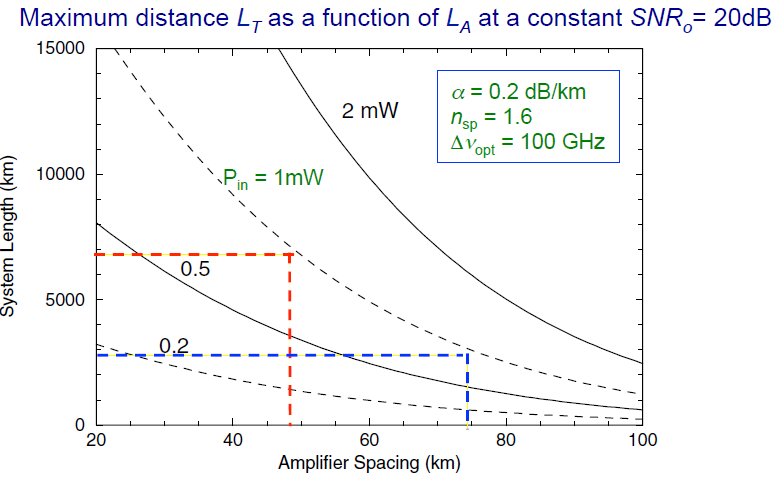
\includegraphics[scale=0.37]{ch6/image16}
	\captionof{figure}{ }
	\end{wrapfigure}
où nous avons utilisé la définition du SNR$_o$ pour la seconde égalité. Cette expression montre que 
le SNR$_o$ augmente rapidement lorsque $M$ est réduite en dessous de 10. La réduction de $M$ impose une 
augmentation de $Q$ pour maintenir un SNR$_o$ constant.\\

En pratique, le SNR$_o$ est supérieur à 20 dB et la puissance maximale est proche de 1 mW à cause des effets
non linéaires (forward mixing). Ceci implique que pour une distance $L_T$, il y a une limite supérieur à 
$L_A$ pour conserver SNR$_o>20$ dB. A titre d'exemple, pour une puissance de l'ordre de 1 mW, pour une
transmission transatlantique (rouge), il faut un amplificateur tous les 50 km. 
\newpage
	\begin{wrapfigure}[14]{l}{8.5cm}
	%\vspace{-5mm}
	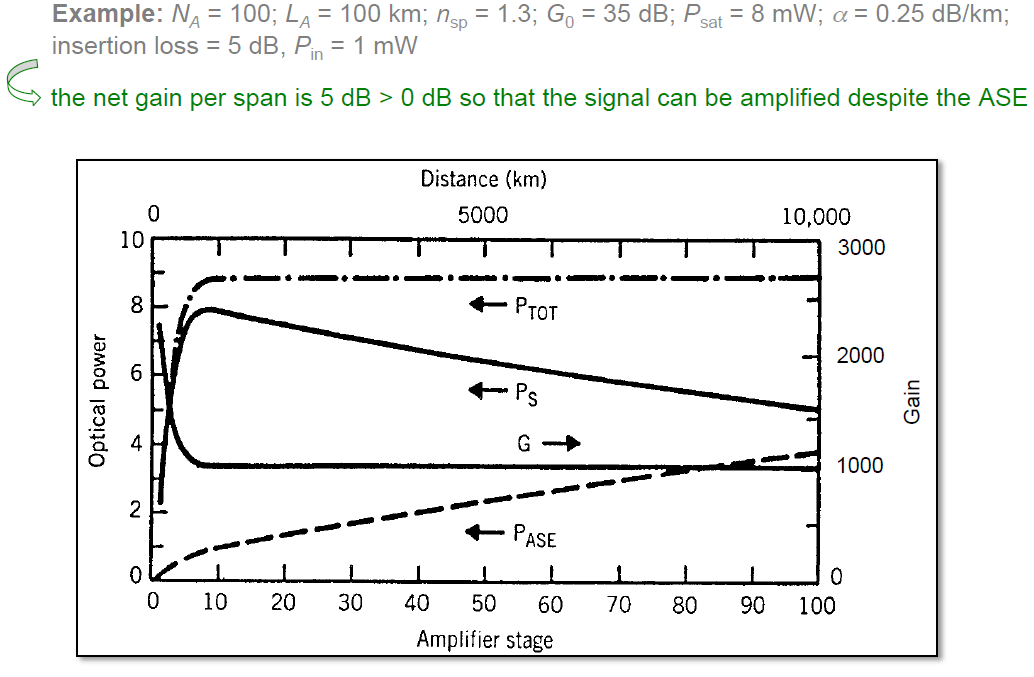
\includegraphics[scale=0.3]{ch6/image17}
	\captionof{figure}{ }
	\end{wrapfigure}


Considérons l'évolution de la puissance du signal et de l'ASE le long d'une chaîne d'amplificateurs 
dopés à l'erbium. On va calculer les pertes juste avant un amplificateur à juste avant le prochain
amplificateur. Les pertes par propagation sont de $100\alpha=25$ dB et les pertes par insertion de 
5 dB, portant les pertes totales à 30 dB ce qui est plus petit que $G_0 = 35$ dB. Si c'était égal, 
l'ASE poserait problème (build-up). La puissance totale va se séparer en $P_S$ + $P_{ASE}$ où 
$P_{ASE}$ ne va faire que augmenter. Si \textit{gain = pertes}, rien de grave pour le premier 
canal. Mais pour le second, on est en présence d'ASE qui va également être amplifiée et le signal 
va déjà commencer à diminuer, d'où l'excès de gain de 5 dB.\\

On voit que la puissance total augmente jusqu'au niveau ou le gain compense les pertes (saturation). 
Ensuite, elle est constante. Rappelons que comme $P_{tot}= c^{te}$ et que $P_{ASE}$ augmente, 
$P_S$ doit forcément diminuer. Au début $P_S$ augmente car excès de gain puis diminue à cause de la
répartion avec l'ASE. Ici le SNR$_o$ est proche de 1 alors qu'il faut au moins 7 : il est très mauvais, 
et la ligne de transmission aussi. Ce n'est pas étonnant car pour une ligne de 10'000km, il faut des
amplificateurs plus fréquemment que ce qui est utilisé ici, à savoir tous les 100km.\\

Le système est donc auto-régulé : après quelques étages, la puissance \textbf{totale} reste constante. La 
puissance totale est telle que la perte par étage est exactement compensée par le gain saturé
\begin{equation}
G = {G_0}\exp [\frac{{1 - G}}{G}.\frac{{{P_s} + {P_{ASE}}}}{{{P_{sat}}}}]
\end{equation}
Même si ce modèle est simple, il permet de trouver la puissance totale
\begin{equation}
{P_{tot}} \approx \ln (\frac{{{G_0}}}{G}){P_{sat}} = {\rm{9}}{\rm{.2 mW}}
\end{equation}

\subsection{Raman amplifiers}
	\begin{wrapfigure}[13]{r}{8cm}
	\vspace{3mm}
	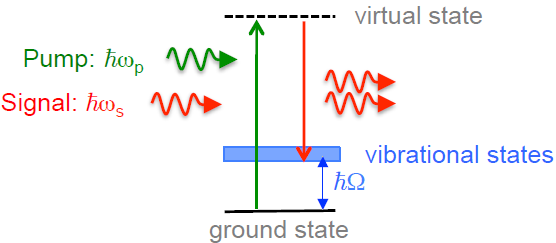
\includegraphics[scale=0.55]{ch6/image18}
	\captionof{figure}{ }
	\end{wrapfigure}
Les amplificateurs Raman fibrés amplifient le signal grâce au \textbf{stimulated Raman scattering} (SRS).
La diffusion de Raman est une diffusion inéalistique dans laquelle un photon est diffusé par une molécule  et
la différence d'énergie entre le photon incident et diffusé excite un état de vibration du système (phonons 
$h\Omega$). Le photon diffusé a donc une énergie ($\hbar\omega_s$) inférieure à l'énergie de la pompe ($\hbar
\omega_p$). Si la différence d'énergie $\hbar\omega_s=\hbar\omega_p-\hbar\Omega$ correspond à l'énergie du signal, celui-ci est amplifié. 
L'étude du spectre Raman permet de retrouver l'emprunte spectrale de la molécule utilisée. 

\newpage

La présence de la pompe et du signal simultanément va causer au battement qui va forcer la molécule à 
vibrer à la différence de fréquence angulaire $\Omega$. Ceci va exciter un état vibrationnel et la différence
d'énergie est un photon supplémentaire pour le signal : transfert d'énergie. Tout se passe donc comme si
l'absorption d'un photon pompe excitait la molécule dans un état virtuel et que, en même temps, le signal photon 
stimule l'émission d'un second photon de signal et la décroissance de la molécule à l'un de ses états 
vibrationnels.

\begin{center}
	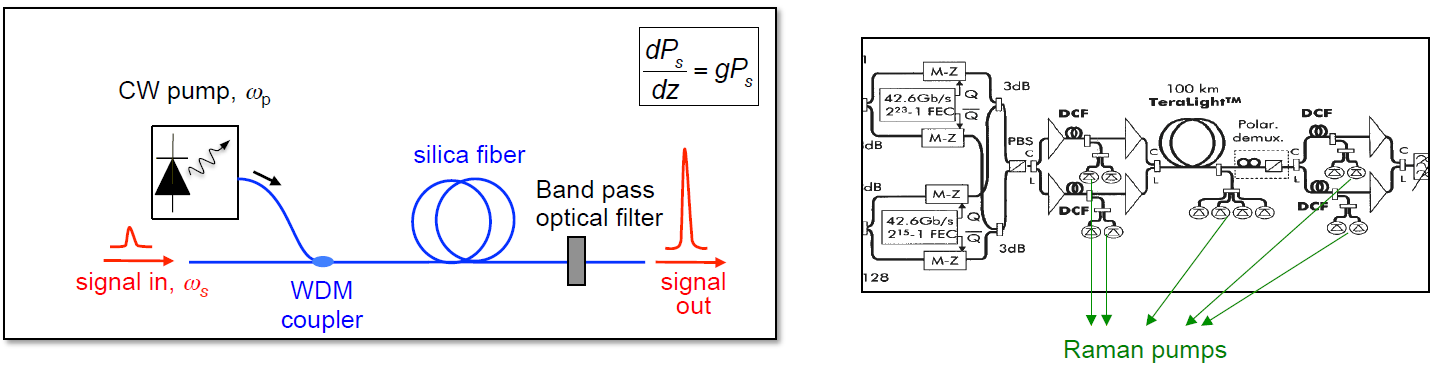
\includegraphics[scale=0.4]{ch6/image19}
	\captionof{figure}{ }
\end{center}

En pratique, les choses sont simples : on prend n'importe quelle fibre et on la pompe. Il faut cependant pas
mal de puissance de pompe, l'effet étant non linéaire. Un WDM est nécessaire car les fréquences sont différentes.


\subsubsection{Raman gain and bandwidth}
	\begin{wrapfigure}[15]{r}{7cm}
	\vspace{-10mm}
	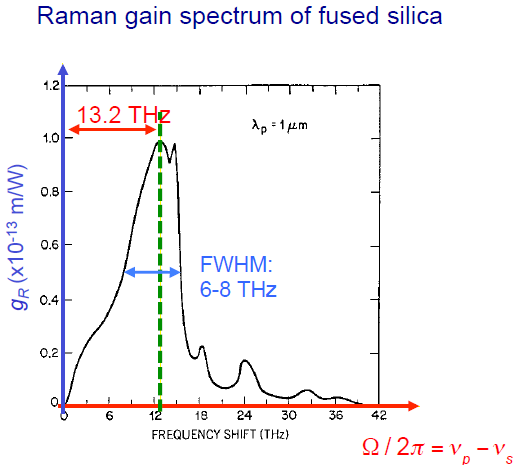
\includegraphics[scale=0.55]{ch6/image20}
	\captionof{figure}{ }
	\end{wrapfigure}
Le gain optique dû au SRS $g$ est lié à l'intensité\footnote{L'effet Raman sera dès lors plus important en 
DCF qu'en SMF.} de la pompe par la relation
\begin{equation}
g = {g_R}{I_p} = {g_R}\frac{{{P_p}}}{{{S_p}}}\qquad\qquad  \frac{{d{P_s}}}{{dz}} = g{P_s}
\end{equation}
$P_p$ la puissance de pompe, $P_s$ la puissance de signal, $S_p$ la surface transverse de la pompe et 
$g_R$ le coefficient de gain Raman. Contrairement à l'amplificateur erbium, l'effet Raman implique un 
niveau virtuel ce qui lève toute dépendance en un matériau. On peut choisir n'importe quelle valeur de pompe, 
il faudra juste faire attention à l'écart pour amplifier correctement le signal. Ci-contre, le gain maximal
est obtenu pour 13.2 ThZ ce qui correspond à l'énergie $\hbar\Omega$.

Le gain Raman dépend de la section transverse de la fibre $g = {g_R}\frac{{{P_p}}}{{{S_p}}}$. Dès lors, 
différentes fibres donnent des gains Raman différents. La force du SRS c'est qu'il existe pour toute les 
longueurs d'onde comme il ne dépend que de la longueur d'onde de pompe. Dès lors, il possède une grande 
largeur à mi-hauteur qui permet d'amplifier sur toute la bande $C$.

\subsubsection{Signal gain in Raman amplifiers}
L'évolution de la puissance du signal et de la pompe s'obtient en résolvant deux équations couplées : la première
pour le signal et la seconde pour la pompe
\begin{equation}
\frac{{d{P_s}}}{{dz}} =  - {\alpha _s}{P_s} + \frac{{{g_R}}}{{{S_p}}}{P_p}\;{P_s},\qquad\qquad
\frac{{d{P_p}}}{{dz}} =  - {\alpha _p}{P_p} - \frac{{{\omega _p}}}{{{\omega _s}}}\frac{{{g_R}}}{{{S_p}}}{P_p}\;{P_s}
\end{equation}
Dans les amplificateurs erbium, très courts, nous pouvions négliger leur pertes mais pas cette fois-ci. Dans 
la limite des petits signaux, le second terme est négligeable : la pompe est si forte que toute sa déplétion 
vient du premier terme. 
\begin{equation}
\frac{{d{P_p}}}{{dz}} \approx  - {\alpha _p}{P_p}\;\; \Rightarrow \;\;\;{P_p}(z) = {P_p}(0)\exp [ - {\alpha _p}z]
\quad\Rightarrow\quad
\frac{{d{P_p}}}{{dz}} \approx  - {\alpha _p}{P_p}\;\; \Rightarrow \;\;\;{P_p}(z) = {P_p}(0)\exp [ - {\alpha _p}z]
\end{equation}
On peut substituer ce résultat dans l'équation du signal et intégrer celle-ci.
\begin{equation}
\int\limits_{{P_s}(0)}^{{P_s}(L)} {\frac{{d{P_s}}}{{{P_s}}}}  = \int\limits_0^L {( - {\alpha _s} + \frac{{{g_R}}}{{{S_p}}}{P_p}(0){e^{ - {\alpha _p}z}})dz} 
\end{equation}
Le résultat de l'intégration donne
\begin{equation}
{P_s}(L) = {P_s}(0)\exp [ - {\alpha _s}L]\exp [\frac{{{g_R}}}{{{S_p}}}{P_p}(0){L_{eff}}]
\end{equation}
où ${L_{eff}} = (1 - {e^{ - {\alpha _p}L}})/{\alpha _p}$. La longueur effective nous informe que l'effet Raman
ne sera présent que sur les premiers kilomètres de la fibre, puis il n'y aura plus de gain. Le facteur
d'amplitication est donné par
\begin{equation}
G(L) = \dfrac{P_S(L)}{P_S(0)}
\end{equation}
Les amplificateurs Raman ont besoin de \textbf{longues fibres} (quelques km) et d'une puissance de pompe
relativement élevées (quelques watts). C'est beaucoup, et c'est ça qui pose des difficultés en pratique : la 
moindre saleté et le connecteur brûle. Les effets non linéaires sont négligeables, $L_{eff}$ étant trop 
"petite". 

\subsubsection{Distributed Raman amplification}
	\begin{wrapfigure}[6]{r}{7cm}
	\vspace{-5mm}
	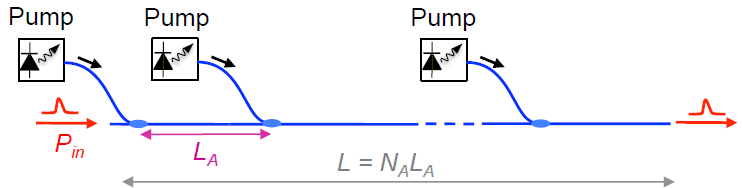
\includegraphics[scale=0.35]{ch6/image21}
	\captionof{figure}{ }
	\end{wrapfigure}
Le gain optique des amplificateurs Raman est considérablement plus petit que celui des EDFA : il est 
nécessaire d'injecter périodiquement de la puissance de pompe dans la fibre. La puissance de pompe 
$P_{in}$ et la distance entre deux stations de pompe $L_A$ est telle que les pertes par propagation 
sont compensées par le gain de chaque étage
\begin{equation}
P_S(L_A)=P_S(L)=P_{in}
\end{equation}
Le SNR$_o$ pour une amplification distribuée est
\begin{equation}
SN{R_o} = \frac{{{P_s}(L)}}{{{N_A}P_{ASE}^{}}} = \frac{{{P_{in}}}}{{2{{\tilde S}_{ASE}}\Delta {\nu _{opt}}{N_a}}}
\end{equation}
Ce n'est pas parce que le niveau est virtuel qu'il n'y a pas de bruit : de l'ASE provient de l'effet Raman
spontané. Cependant, le bruit est faible car l'absorption des photons du signal dans l'état virtuel "haut" 
est très faible\footnote{"\textit{La principale différence entre les amplificateurs Raman et les EDFA est que ces derniers sont à faible bruit. Le facteur d'émission spontanée des EDFA dépend en effet de l'inversion de population et donc de la puissance de la pompe. Pour une puissance de pompe faible, le gain local net peut être négatif. Cependant, même pour une faible puissance de pompage, il y a toujours des émissions spontanées car la population de l'état supérieur est non nulle. Au contraire, les amplificateurs Raman sont peu bruyants quelle que soit la puissance de la pompe car l'absorption des photons du signal vers l'état virtuel supérieur est extrêmement faible. Le gain reste donc toujours positif lorsqu'une diffusion Raman spontanée non négligeable de la pompe se produit.
}"}.

\newpage
	\begin{wrapfigure}[8]{r}{7cm}
%	\vspace{-5mm}
	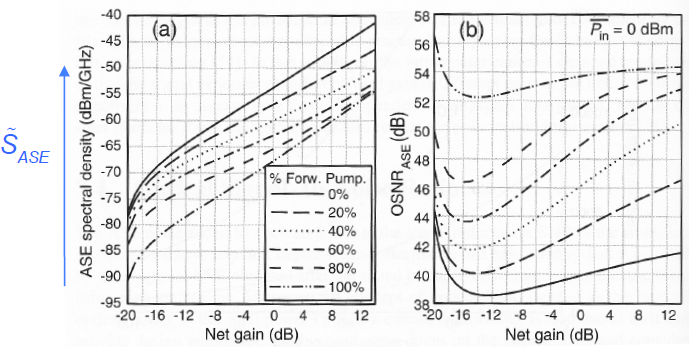
\includegraphics[scale=0.35]{ch6/image22}
	\captionof{figure}{ }
	\end{wrapfigure}
Dans le cas d'amplificateurs Raman distribués, $L=100$km et $P_{in}=1$mW, les performances sont meilleurs 
que dans le cas simplement pompé (forward). Pour une système à $L=10000$km, SNR$_o\approx50-20=30$ dB (50 pour
un ampli, 20 pour la cascade). C'est mieux que les 20 dB requis et très différent de l'erbium ou le SNR$_o$ 
est proche de 1.  Ici, on peut en mettre tous les 100km. On les utilise aujourd'hui car ils ont un bruit
plus faible que l'EDFA.


\subsubsection{Systems using backward pumping distributed Raman amplification to assist in the amplification}
En envoyant la pompe Raman vers l'arrière à chaque phase d'amplification, l'amplification Raman distribuée permet à l'amplitude du signal de rester en dessous du niveau des effets non linéaires puisque l'amplification du signal le long de la seconde moitié maintient l'émission au-dessus du bruit sol.
\begin{center}
	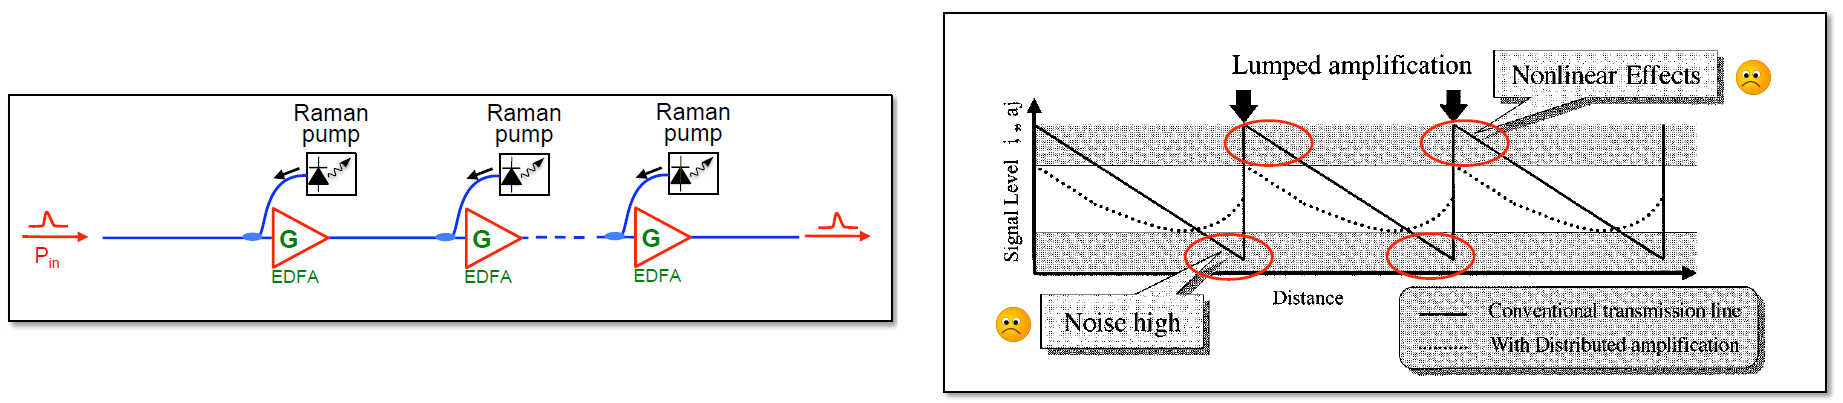
\includegraphics[scale=0.3]{ch6/image23}
	\captionof{figure}{ }
\end{center}

\section{Nonlinear effects in optical fibers}
\subsection{Introduction}
Augmenter la puissance d'un signal permet la propagation sur des distances plus importantes. Cependant, si la
puissance devient trop importante, les interactions non linéaires entre la silice et le signal deviennent non 
négligeable (de même si la longueur de propagation augmente). Des effets non linéaires variés peuvent apparaître
dans les système à simple ou multiple channel : \textbf{limite supérieure} à la puissance. Par contre, les
performances sont dégradées lorsque le SNR$_o$ est trop faible au récepteur : \textbf{limite inférieure} à la
puissance.\\

Il y a donc un compromis entre le signal minimum (limite le bruit) et le maximum (limite effets non linéaires).
Les effets peuvent être catégorisés en processus de diffusion ou en processus lié à l'effet Kerr. Plusieurs facteurs
influences ces effet.
\begin{center}
	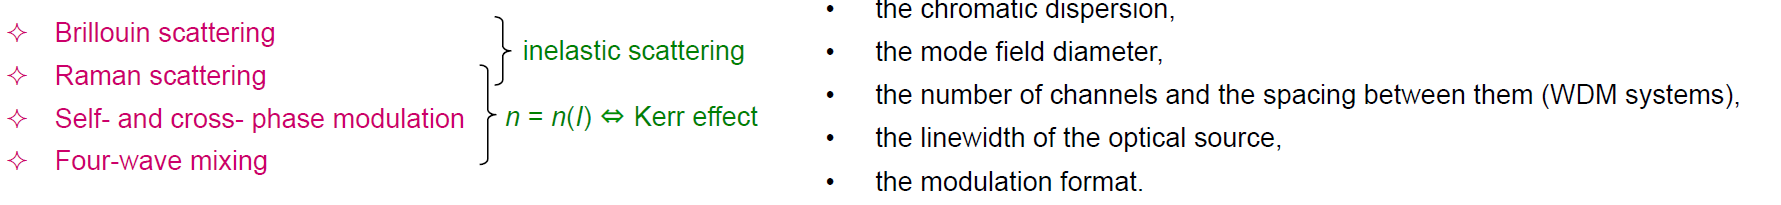
\includegraphics[scale=0.3]{ch6/image24}
	\captionof{figure}{ }
\end{center}
\newpage

\subsection{Brillouin scattering}
L'origine physique de la \textbf{diffusion de Brillouin} est un phénomène 
d'\textit{électro-striction} : la tendance d'un matériau à être compressé en présence d'un champ
électrique. Le matériau devient plus dense lorsque la densité d'énergie électromagnétique augmente. 
Pour une onde électromagnétique de fréquence $\omega_p$, ce phénomène génère une onde acoustique
de fréquence $\Omega$. \\

	\begin{wrapfigure}[6]{r}{7cm}
	\vspace{-5mm}
	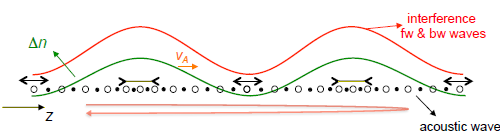
\includegraphics[scale=0.5]{ch6/image25}
	\captionof{figure}{ }
	\end{wrapfigure}
Comme le matériau est compressé\footnote{Il s'agit bien de la génération d'un phonon sur la bande
acoustique alors que l'effet Raman est plus lié à l'optique.}, son indice de réfraction augmente par 
\textit{effet photo-élastique} et la lumière est diffusée par la variation d'indice de réfraction. 
Celle-ci va interférer avec la lumière incidente : patern d'interférence. Il va donner lieu à 
l'apparition d'un réseau d'indice de réfraction mobile (l'onde accoustique) qui cause lui-même 
de la diffusion.\\

\textbf{La diffusion de Brillouin spontanée} peut être vue comme la diffusion de l'onde à 
$\omega_p$ sur l'onde acoustique. Ce processus de diffusion inélastique génère une nouvelle onde
à fréquence $\omega_s=\omega_p-\Omega$ où $\Omega$ est la fréquence associée au phonon.\\

	\begin{wrapfigure}[6]{l}{7cm}
	\vspace{-5mm}
	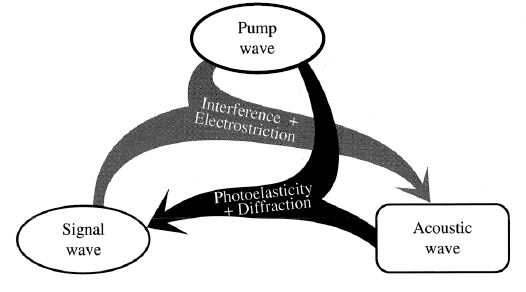
\includegraphics[scale=0.4]{ch6/image26}
	\captionof{figure}{ }
	\end{wrapfigure}
\textbf{La diffusion de Brillouin stimulée} (SBS) se produit lorsque le battement entre l'onde
initiale $\omega_p$ et l'onde diffusée $\omega_s$ renforcent l'onde acoustique ($\Omega =
\omega_p-\omega_s$) par électro-striction\footnote{QR !}.\\

Par conservation de l'énergie et de l'impulsion
\begin{equation}
\hbar {\omega _p} = \hbar {\omega _s} + \hbar \Omega ,\qquad\qquad
\hbar {k_p} = \hbar {k_s} + \hbar q
\end{equation}
On retrouve bien une partie de l'énergie de la pompe diffusée et l'autre partie génère l'onde
acoustique. Dans une fibre optique, seule les modes forward ($+z, \theta=0$) et 
backward ($-z, \theta=\pi$) peuvent se propager. Il y a donc deux directions pour $\vec{k_s}$. 
De plus
\begin{equation}
q_\perp = q\sin(\theta')= 0\qquad\Rightarrow\qquad \theta'=0
\end{equation}
On en déduit
\begin{equation}
k_p \pm k_s = q
\end{equation}
où il faudra considérer $\pm k_s$ selon le sens de diffusion et où $q$ est le nombre d'onde 
du vecteur créé. Comme $\Omega = qv_a$ 
\begin{equation}
 \Rightarrow \Omega  = ({k_p} \pm {k_s}){v_A} = {k_p}{v_A}(1 \pm \frac{{{k_s}}}{{{k_p}}})
\end{equation}
où $v_a$ est la vitesse de l'onde acoustique. Sachant que
\begin{equation}
\frac{{{k_s}}}{{{k_p}}} = \frac{{{\omega _s}}}{{{\omega _p}}} = \frac{{{\omega _p} - \Omega }}{{{\omega _p}}} = 1 - \frac{\Omega }{{{\omega _p}}} = 1 - \frac{q}{{{k_p}}}\frac{{{v_A}}}{{c/{n_{eff}}}} \approx 1
\end{equation}
En effet, $q/k_p\to 1$ (même ordre de grandeur que dans l'optique) par contre $v_a/c\to0$. Donc
\begin{equation}
\Omega  = {k_p}{v_A}(1 \pm 1)
\end{equation}
Si $\theta=0$ ; diffusion inélastique dans la même direction, impliquant $\Omega=0$ (le phonon
ne prend pas d'énergie). Si par contre le photo est rétro-diffusé ($\theta=\pi$), $\Omega = 
2k_pv_a$. On en conclu que le SBS ne se produit que en \textbf{rétro-diffusion}. Le saut de
fréquence est\footnote{??}
\begin{equation}
{\nu _B} = \frac{{2{k_p}{v_A}}}{{2\pi }} = \frac{{2{n_p}{v_A}}}{{{\lambda _p}}} \approx 11\;\;GHz
\end{equation}
pour $v_a\approx5.9$km. La fréquence de l'onde diffusée est presque identique à celle du signal
d'entrée. Il y a un \textbf{seuil de puissance} au delà duquel presque toute la puissance 
incidente est transférée à l'onde diffusée par SBS. Ce seuil dépend de la fibre, mais aussi
de la largeur de la source laser \textbf{et} du format de modulation.\\

\begin{wrapfigure}[7]{r}{7cm}
	\vspace{-5mm}
	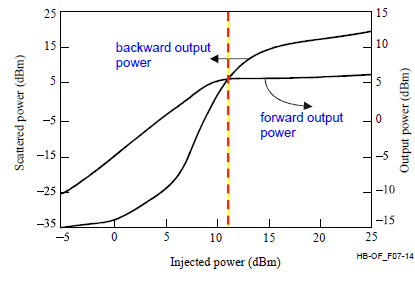
\includegraphics[scale=0.55]{ch6/image27}
	\captionof{figure}{ }
	\end{wrapfigure}
	
La largeur de gain du SBS est liée au temps d'amortissement de l'onde acoustique. Il est de
l'ordre de $50 MHz$ dans une fibre en silice à 1.55 $\mu$m. Ainsi, cet effet ne va pas
fortement dégrader les performances du système \footnote{Comprends pas la conclusion}

\begin{itemize}
\item[$\bullet$] Lorsque la largeur de bande de la porteuse est grande par rapport à 50 MHz ou 
avec une modulation de phase.
\item[$\bullet$] Quand la puissance est en dessous du seuil (quelques mW). 
\end{itemize}


\subsection{Stimulated Raman scattering}
\begin{wrapfigure}[7]{l}{8cm}
	\vspace{-5mm}
	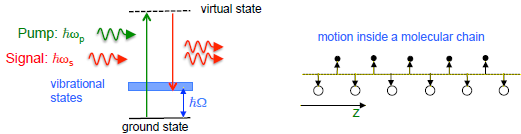
\includegraphics[scale=0.55]{ch6/image28}
	\captionof{figure}{ }
	\end{wrapfigure}
Le principe physique derrière la diffusion de Raman est le transfert d'énergie aux molécules
de silice et plus précisément, aux états vibrationnels. Considérons une chaîne d'atomes. La
diffusion Raman est une excitation non pas longitudinale, mais transverse (à fréquence plus
élevée que la diffusion Brillouin, 13 THz contre 11 GHz). La grande différence avec Brillouin
est que cette diffusion peut se faire en forward et en backward\footnote{Pas d'onde acoustique
sujette au phase matching.}. A cause de la structure amorphe du verre, la bande passante de 
la diffusion Raman est grande ($\Delta \nu \approx 6-8$ THz). La \textbf{diffusion stimulée 
Raman} (SRS) affecte les systèmes simple/multi-channels. 


\subsubsection{Single-channel systems}
\begin{wrapfigure}[7]{r}{4cm}
	\vspace{-5mm}
	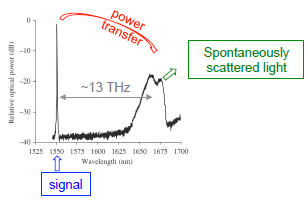
\includegraphics[scale=0.55]{ch6/image29}
	\captionof{figure}{ }
	\end{wrapfigure}
Dans de tel système\footnote{Nuance canaux/monocrhoma. Pulse ? D'accord que WDM on mix bcp de lambda
mais fibre monomode pour chacun d'eux?}, la diffusion de Raman peut
causer une atténuation de la puissance signal. En effet, le signal \textbf{joue la pompe} pour
l'amplification des photons générés par SRS ainsi que l'amplification du bruit généré par les
amplificateurs \textit{inline}. Cependant, sans amplificateurs, on doit injecter $\approx$ 500
mW pour l'observer : c'est gigantesque, elle ne posera pas de problèmes. 

\newpage
\subsubsection{Multichannel systems}
\begin{wrapfigure}[7]{l}{8cm}
	\vspace{-5mm}
	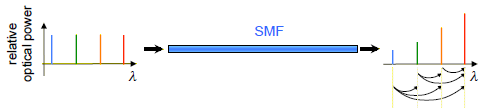
\includegraphics[scale=0.55]{ch6/image30}
	\captionof{figure}{ }
	\end{wrapfigure}
Avec la SRS, le \textbf{signal} à la longueur d'onde $\lambda_s$ devient une \textbf{pompe Raman} 
pour les canaux à d'autres longueurs d'onde : transfert d'énergie les petites longueurs d'onde
vers les grandes. La SRS dégrade les systèmes WDM : déplétion du signal et crosstalk.\\

A cause de cet effet, il faut augmenter la pénalité en puissance pour maintenir le facteur de 
qualité voulu. Par exemple (voir \textit{slide 65}), on est limite à une vingtaine de canaux à
10 mW.\\

Raman implique une pénalité de puissance dans la puissance par canal $P_{ch}$, le nombre de 
canaux $N_{ch}$ et l'espace inter-canaux $\Delta \nu_{ch}$. A cause des pertes, l'effet n'est
à prendre en considération sur une distance de $L_{eff}=[1-\exp(-\alpha L)]/\alpha$ ainsi 
que la surface effective du mode dans la fibre $S$. Il en résulte une sorte de formule
empirique\\

\cadre{\begin{equation}
{P_{tot}}\Delta \lambda {L_{eff}} < 40\;{\rm{mW}}{\rm{.nm}}{\rm{.Mm}}
\end{equation}
où $P_{tot} = N_{ch}P_{ch}$, $\Delta \lambda = N_{ch}\Delta\lambda_{ch}$ et 
$L_{eff}\approx1/\alpha$.}\ \\

Cette relation permet, si une pénalité de puissance de 1 dB est acceptable, d'estimer le seuil
de puissance total $P_{tot}$ causé par la SRS. 


\subsection{Nonlinear polarization}
Dans l'approche électromagnétique des guides d'onde, les interactions optiques étaient supposées
linéaires : les interactions lumière-matières sont décrites par la polarisation linéaire
\begin{equation}
\vec{P}\left( {{\bf{r}},t} \right) = {\varepsilon _0}\int_{ - \infty }^{ + \infty } {\chi \left( {{\bf{r}}',t - t'} \right)}  \vdots \vec{E}\left( {{\bf{r}},t'} \right)dt'.
\end{equation}
Pour un milieu isotropique avec une réponse instantanée et locale
\begin{equation}
\chi \left( {{\bf{r}},{t_0}} \right) = \tilde \chi \left( {\bf{r}} \right)\delta \left( {t - {t_0}} \right)\qquad\Rightarrow\qquad \vec{P}\left( {{\bf{r}},t} \right) = {\varepsilon _0}\tilde \chi \vec{E}\left( {{\bf{r}},t} \right)
\end{equation}
Ceci est indépendant de la fréquence (instantané). Pour des champs électrique important, la
polarisation n'est plus juste proportionnelle à l'amplitude du champ électrique. C'est le 
régime de propagation non linéaire. Lorsqu'on se situe loin des transition d'énergie entre
deux niveaux\footnote{Soit les résonance, pour les fibres optiques loin de l'UV et l'IR moyen}
\begin{equation}
\vec{P} = {\varepsilon _0}{\tilde \chi ^{(1)}}\vec{E} + {\varepsilon _0}{\tilde \chi ^{(2)}}{\vec{E}^2}\vec{ + }{\varepsilon _0}{\tilde \chi ^{(3)}}{\vec{E}^3}\vec{ + } \cdots 
\end{equation}
Dans la fibre optique, $\chi^{(2)}=0$. Le plus bas ordre de polarisation non linéaire est donc
\begin{equation}
{\vec{P}_{nl}} = {\varepsilon _0}{\tilde \chi ^{(3)}}{\vec{E}^3}
\end{equation}
Considérons donc 
\begin{equation}
P = {\varepsilon _0}{\tilde \chi ^{(1)}}E + {\varepsilon _0}{\tilde \chi ^{(3)}}{E^3}
\end{equation}
avec $\DS E = E{e^{j{\omega _0}t}} + {E^*}{e^{ - j{\omega _0}t}} $. Développons le cube du champ
 électrique
\begin{equation}
\begin{array}{ll}
{E^3} &\DS= ({E^2}{e^{j2{\omega _0}t}} + {E^{*2}}{e^{ - j2{\omega _0}t}} + 2E{^2})(E{e^{j{\omega _0}t}} + {E^*}{e^{ - j{\omega _0}t}})\vspace{2mm}\\
&\DS= ({E^3}{e^{j3{\omega _0}t}} + {E^{*3}}{e^{ - j3{\omega _0}t}} + {E^2}{E^*}{e^{j{\omega _0}t}} + E{E^{*2}}{e^{ - j{\omega _0}t}}\; + 2E{^2}E{e^{j{\omega _0}t}} + 2E{^2}{E^*}{e^{ - j{\omega _0}t}})
\end{array}
\end{equation}
La polarisation s'écrit
\begin{equation}
P = {\varepsilon _0}{\tilde \chi ^{(1)}}E{e^{j{\omega _0}t}} + {\varepsilon _0}{\tilde \chi ^{(3)}}({E^3}{e^{j3{\omega _0}t}} + 3E{^2}E{e^{j{\omega _0}t}}) + c.c
\end{equation}
On voit apparaître un terme source : il s'agit de la \textbf{troisième harmonique}, qui peut être
ignorée dans les fibres optiques (pas de \textit{phase-matching}). Si l'on réécrit la polarisation 
$P = P{e^{j{\omega _0}t}} + {P^*}{e^{ - j{\omega _0}t}}$, on en tire
\begin{equation}
P = {\varepsilon _0}({\tilde \chi ^{(1)}} + 3E{^2}{\tilde \chi ^{(3)}})E
\qquad\Rightarrow\qquad
 P_{nl}^{{\omega _0}} = 3{\varepsilon _0}{\tilde \chi ^{(3)}}E{^2}E
\end{equation}
Il s'agit de l'\textbf{effet Kerr}.

\subsection{Self-phase modulation (SPM)}
Considérons le régime de propagation non linéaire $P = {\varepsilon _0}({\tilde \chi ^{(1)}} + 3E{^2}
{\tilde \chi ^{(3)}})E$. La susceptibilité (non linéaire) vaut $\tilde \chi  = {\tilde \chi ^{(1)}} +
 3E{^2}{\tilde \chi ^{(3)}}$. Par la définition conventionnelle de l'indice de réfraction
\begin{equation}
n = \sqrt {1 + \tilde \chi }  = \sqrt {1 + {{\tilde \chi }^{(1)}} + 3{{\tilde \chi }^{(3)}}E{^2}}  = \sqrt {n_0^2 + 3{{\tilde \chi }^{(3)}}E{^2}}  \approx {n_0} + \frac{{3{{\tilde \chi }^{(3)}}E{^2}}}{{2{n_0}}}
\end{equation}
où $n_0$ est l'indice de réfraction linéaire. Nous allons considérer qu'on ne lui ajoute qu'une
perturbation de sorte à le mettre en évidence et obtenir la dernière "égalité". Nous allons 
considérer que ce sont des scalaires\footnote{Pas très "grave" pour les fibres optiques.}. 
L'amplitude du champ analytique est lié à l'intensité par la relation $E{^2} = I/(2{\varepsilon _0}
c{n_0})$. En utilisant notre expression de $n$, on trouve l'\textbf{effet Kerr optique}\\

\cadre{\begin{equation}
n = {n_0} + n_2^II \qquad\text{ où}\quad n_2^I = \frac{{3{{\tilde \chi }^{(3)}}}}{{4{\varepsilon _0}cn_0^2}} \text{ (indice de réfraction NL)}
\end{equation}}\ \\

L'indice de réfraction va ainsi varier en fonction de l'intensité. Dans la fibre optique, on 
remplace l'intensité par la puissance transportée par le mode fondamental $I=PS$, où $S$ est
la surface effective du mode fondamental. \textbf{L'effet Kerr linéaire modifie la constante
de propagation}
\begin{equation}
\beta  = \frac{{2\pi }}{\lambda }({n_0} + n_2^I\frac{P}{S}) = {\beta _0} + \frac{{2\pi n_2^I}}{{\lambda S}}P = {\beta _0} + \gamma P
\end{equation}
où $\beta_0$ est la constante de propagation du mode guidé et $\DS \gamma  \equiv \frac{{2\pi n_2^I}}
{{\lambda S}}$.\\

\subsubsection{Nonlinear propagation equation}
Au chapitre 2, nous avons dérivé la relation de dispersion
\begin{equation}
\beta \left( \omega  \right) \approx {\beta _0} + {\beta _1}\left( {\omega  - {\omega _0}} \right) +
 \frac{1}{2}{\beta _2}{\left( {\omega  - {\omega _0}} \right)^2} + \dots
\end{equation}
avec $E(\rho ,\theta ,z,t) = F(\rho ,\theta )A(z,t).\exp \left( {j[{\omega _0}t - {\beta _0}z]}
 \right)$. Nous avions alors trouvé
 \begin{equation}
\frac{{\partial A}}{{\partial z}} - j\frac{{{\beta _2}}}{2}\frac{{{\partial ^2}A}}{{\partial {t^2}}} + \dots = 0
 \end{equation}
Étudions maintenant la propagation d'un pulse d'amplitude $A_0(t)$ dans le régime non linéaire
\begin{equation}
{\beta _0} \to {\beta _0} + \gamma P\qquad\Rightarrow\qquad A = {A_0}(t){e^{ - j\gamma P(t)z}}
\end{equation}
où $P(t)\propto |A(t)|^2$. L'amplitude $A$ obéit à l'équation
\begin{equation}
\frac{{\partial A}}{{\partial z}} + j\gamma PA = 0
\end{equation}
En prenant en compote la GVD et en sommant les deux, on trouve l'\textbf{équation de Schrödinger
non linéaire} (NLS)\\

\cadre{\begin{equation}
\frac{{\partial A(z,t)}}{{\partial z}} - j\frac{{{\beta _2}}}{2}\frac{{{\partial ^2}A}}{{\partial {t^2}}} + j\gamma A{^2}A = 0
\end{equation}}\ \\

\begin{wrapfigure}[7]{l}{5cm}
	\vspace{-5mm}
	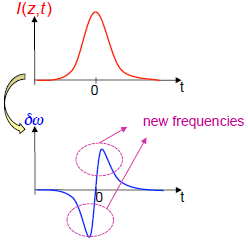
\includegraphics[scale=0.65]{ch6/image31}
	\captionof{figure}{ }
	\end{wrapfigure}
Supposons qu'il n'y ai pas de dispersion ($\beta_2=0$)
\begin{equation}
\frac{{\partial A}}{{\partial z}} + j\gamma PA = 0\qquad\Rightarrow\qquad
A(z,t) = A(0,t){e^{ - j\gamma A(z,t){^2}z}}
\end{equation}
On voit que le champ électromagnétique modifie lui même sa propre phase : c'est 
l'\textbf{auto-modulation de phase}. La phase n'est plus linéaire, elle vaut
\begin{equation}
 \Rightarrow \;\;{\varphi _{nl}}(z,t) =  - \gamma A(z,t){^2}z
\end{equation}\ \\

Il lui correspond donc un chirp
\begin{equation}
\delta \omega  = \frac{{\partial {\varphi _{nl}}}}{{\partial t}} =  - \gamma \frac{{\partial A(z,t){^2}}}{{\partial t}}z
\end{equation}
Au maxima, la dérivée est nulle. Par contre, sur les flancs montants et descandents elle ne l'est pas
et on va générer de nouvelle fréquence. La non linéarité ajoute de \textbf{nouvelles} fréquences 
qui causeront de la distorsion (le spectre est ainsi élargi).

\begin{center}
	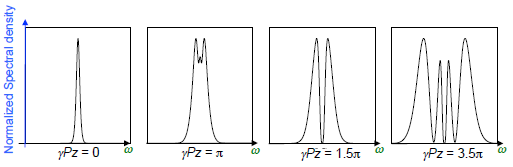
\includegraphics[scale=0.65]{ch6/image32}
	\captionof{figure}{Spectre pour différentes valeurs de $z$, dans un milieu sans pertes.}
\end{center}

On voit que la fréquence initiale a été entièrement convertie. En continuant la propagation, 
on va "creuser" les nouvelles fréquences et ainsi de suite. La SPM augmente lorsque la puissance
augmente ainsi que le bit rate (pentes plus raides). La SPM est négative dans les \textit{long-haul
system}  (effets cumulatif et dispersion chromatique) et dans les systèmes DWDM (interférence entre
canaux adjascents (inter-channel crosstalk)).

\newpage
Dans les fibre optique, la puissance évolue comme ($\alpha\neq 0$) $P(z) = P(0){e^{ - \alpha z}}$. 
Comme la phase dépend de la puissance, elle sera maximale pour
\begin{equation}
{\varphi _{nl,\max }} =  - \int\limits_0^L {\gamma {{\left| {A(z)} \right|}^2}dz} 
 =  - \int\limits_0^L {\gamma P(0){e^{ - \alpha z}}dz = }  - \gamma P(0){L_{eff}}
\end{equation}
où ${L_{eff}} = [1 - \exp ( - \alpha L)]/\alpha $. Il s'agit de la longueur sur laquelle on
peut observer des effets non linéaire. Au delà, la puissance est trop faible. On n'observera
ces effets qu'en début de ligne, sau si on place des amplificateurs (la, on aura la chance de 
retrouver à chaque fois la SPM).\\

Si une phase non linéaire de 0.1 est acceptable, la puissance d'entrée est limitée (pour 
$N_a$ étages d'amplification)
\begin{equation}
P(0) < \frac{{0.1\alpha }}{{\gamma {N_a}}}
\end{equation}
Si l'on module en phase, la puissance reste constante $P(t)=P_0$ : shift constant causé par la
SPM et pas d'élargissement spectral.


\subsection{Cross-phase modulation (XPM)}
Il s'agit ici d'influence de phase pour des signaux qui n'ont pas la même longueur d'onde (système
WDM). Considérons un champ électromagnétique composé de deux ondes, une à $\omega_1$ et l'autre
à $\omega_2$
\begin{equation}
E = {E_1}{e^{j({\omega _1} - {\omega _0})t}} + {E_2}{e^{j({\omega _2} - {\omega _0})t}}
\end{equation}
On peut en déduire (comme dans la section sur la polarisation non linéaire, section 6.2.3) les 
polarisation des deux ondes
\begin{equation}
\begin{array}{lll}
P_{nl}^{{\omega _1}} &\DS= 3{\varepsilon _0}{\tilde \chi ^{(3)}}({E_1}{^2} + 2{E_2}{^2}){E_1}
&\DS\Rightarrow \;\;\Delta \varphi _{nl}^{{\omega _1}} =  - \gamma {L_{eff}}(\;\underline{P_1}\; + \;\underline{\underline{2P_2}}\;)\;
\vspace{2mm}\\
P_{nl}^{{\omega _2}}&\DS= 3{\varepsilon _0}{\tilde \chi ^{(3)}}({E_2}{^2} + 2{E_1}{^2}){E_2}&\DS
\Rightarrow \;\;\Delta \varphi _{nl}^{{\omega _2}} =  - \gamma {L_{eff}}(\;\underline{P_2}\; + \;\underline{\underline{{2P_1}}}\;)
\end{array}
\end{equation}
On observe de l'\underline{auto-modulation de phase} mais également 
de la \underline{\underline{modulation de phase croisée}} (XPM). Cet effet est responsable 
d'un élargissement du spectre en OOK. Le bit '1' du signal à $\omega_1$ va influencer
le bit '1' du signal à $\omega_2$ (car énergie) et il va en résulter un élargissement spectral. Il
s'agit d'un effet de pure modulation de phase mais qui ajoute de nouvelle fréquence, causant un
élargissement spatial de l'impulsion\footnote{Heuuu}. On voit qu'on a intérêt à utiliser des
fibres avec une certaine dispersion pour éviter de "croiser les '1'.


\subsection{Four-wave mixing (FWM)}
\begin{wrapfigure}[7]{l}{9cm}
	\vspace{-5mm}
	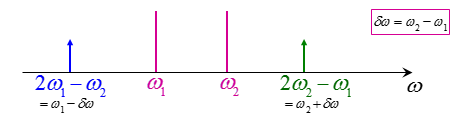
\includegraphics[scale=0.65]{ch6/image33}
	\captionof{figure}{ }
	\end{wrapfigure}
Considérons deux signaux ($\omega_1, \omega_2$)
\begin{equation}
E = {E_1}{e^{j({\omega _1} - {\omega _0})t}} + {E_2}{e^{j({\omega _2} - {\omega _0})t}}
\end{equation}
Le calcul de la polarisation fait apparaître deux termes à fréquence nouvelle
\begin{equation}
P_{nl}^{2{\omega _1} - {\omega _2}} = 3{\varepsilon _0}{\tilde \chi ^{(3)}}E_1^2E_2^*,\qquad\qquad
P_{nl}^{2{\omega _2} - {\omega _1}} = 3{\varepsilon _0}{\tilde \chi ^{(3)}}E_2^2E_1^*
\end{equation}
Le \textbf{mélange à quatre ondes} (FWM) est responsable d'un \textbf{transfert d'énergie} de 
deux ondes à $\omega_1$ et $\omega_2$ vers deux autres ondes à $2\omega_1-\omega_2$ et 
$2\omega_2-\omega_1$.

\newpage
\begin{wrapfigure}[7]{l}{7.5cm}
%	\vspace{-5mm}
	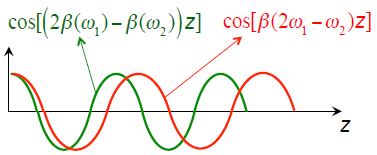
\includegraphics[scale=0.65]{ch6/image34}
	\captionof{figure}{ }
	\end{wrapfigure}
Il existe un mécanisme pour éviter ces échanges d'énergie : c'est la dispersion chromatique. 
Considérons le cas précédent du mélange à quatre onde en nous intéressant plus particulièrement
à l'onde de fréquence $2\omega_1-\omega_2$. Sa polarisation et son champ sont donnés par\\

\begin{equation}
P_{nl}^{2{\omega _1} - {\omega _2}}(z) \propto A_1^2A_2^*{e^{ - j[2\beta ({\omega _1}) - \beta ({\omega _2})]z}}\qquad\qquad
{E_{2{\omega _1} - {\omega _2}}}(z) \propto {e^{ - j\beta (2{\omega _1}\; - \;{\omega _2})z}}
\end{equation}
Or, rien ne dit que les exponentielles sont égales.  En vert, le champ de polarisation. Il peut
être un terme source pour le rouge mais il possède une autre constante : à un certain moment, 
les champs seront en opposition. Il faut qu'ils soient en phase pour devenir macroscopique 
(sinon ne respecte pas la conservation de l'impulsion). Le champ à $2\omega_-\omega_2$ grandira
seulement si
\begin{equation}
\beta (2{\omega _1}\; - \;{\omega _2}) \approx 2\beta ({\omega _1}) - \beta (\;{\omega _2})
\end{equation}
Soit un (quasi-)respect de la conservation de l'impulsion. On parle de \textbf{condition de 
phase matching}. On peut développer en série (voir \textit{slide 78}) pour réécrire la condition 
de phase matching
\begin{equation}
\frac{1}{2}\delta {\omega ^2}\beta ''({\omega _1}) + 4\gamma P \approx 3\gamma P - \frac{1}{2}\delta {\omega ^2}\beta ''({\omega _1})\qquad\Leftrightarrow\qquad
 - \delta {\omega ^2}\beta ''({\omega _1}) \approx \gamma P
\end{equation}
A gauche la dispersion chromatique, à droite la non-linéarité de la fibre et la puissance du 
signal. L'adaptation de puissance permet l'obtention d'un transfert d'énergie efficace. Il est
indispensable de vérifier cette condition (qui dépend de $\beta''$ et $\gamma P$) pour voir le
résultat du mélange à quatre ondes\footnote{Pourquoi 4 ? On n'en verra jamais que 3 au mieux, non?}.\\

Le FWM est un processus non linéaire dans laquelle une interaction avec deux ou trois ondes génère
de nouvelles ondes à fréquences différentes ($\omega_4=\omega_1\pm\omega_2\pm\omega_3$). Pour
des canaux également espacés, avec la même puissance, le FWM est efficace sur la bande passante
\begin{equation}
[\delta {\omega ^2}\beta ''] \approx \gamma P
\end{equation}
Près du zéro de dispersion $\beta''\approx0$, le FMW est efficace même entre des canaux loin
les un des autres\footnote{?}. Le FWM cause un transfert d'énergie entre les canaux voisins les
plus proches (perte de puissance dans le canal, inter-channel crosstalk (fluctuation amplitude
'1')). L'efficacité du FWM est réduite en espaçant les canaux ou en les espaçant de façon
inégales (pas utilisé en pratique).

\subsection{Dispersion map}
Les effets non linéaires croisés sont responsable d'un crosstalk inter-canaux. On peut réduire
ces effets en maintenant localement une grande dispersion chromatique pour que la vitesse de groupe
soit différente sur chaque canal (mais il faudra la compenser à la fin). Cependant, la dispersion
chromatique dégrade des performances quand elle n'est pas proprement compensée. On utilise alors des
NZDSF ou on compense dans le récepteur. \\

\newpage
\begin{wrapfigure}[12]{l}{6cm}
%	\vspace{-5mm}
	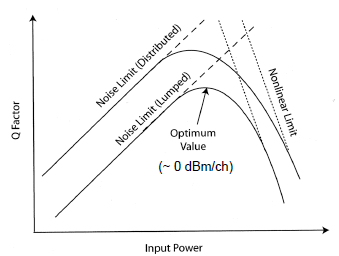
\includegraphics[scale=0.65]{ch6/image35}
	\captionof{figure}{ }
	\end{wrapfigure}
On se rappelle que l'élargissement temporel était donné par
\begin{equation}
\Delta T = \sum\limits_j {{L_j}{D_j}} \Delta \lambda 
\end{equation}
Les valeurs de $L_j$ et $D_j$ forment la carte de dispersion. Dans un régime linéaire, l'ordre
n'a pas d'importance mais en non linéaire, il peut en avoir! En effet, la dispersion interagit avec
les effets non linéaires : le facteur de qualité dépend de la variation de dispersion le long
de la ligne, ce qui est indiqué par la \textbf{dispersion map}. Les \textit{slides 82} à 
\textit{83} illustrent ces propos. 

\subsection{Optimal input power}
Comme dit en début de section, il y a un compromis entre les grand effets non linéaires au cours
de la propagation et la dégradation du SNR$_o$ par les amplificateurs.\footnote{Ndlr : j'ai passé
quelques développements mathématiques dans cette section. Une lecture des slides devrait cependant
être suffisante (mais il \textbf{faut} le faire).}

\section{Coherent systems}
\subsection{Introduction}
\begin{wrapfigure}[10]{l}{7cm}
	\vspace{-5mm}
	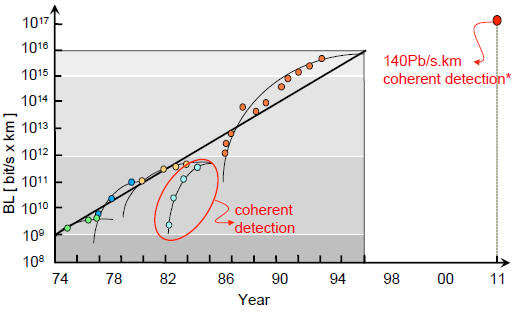
\includegraphics[scale=0.45]{ch6/image36}
	\captionof{figure}{ }
	\end{wrapfigure}
Le produit $BL$ n'a cessé d'augmenter depuis la création de la fibre optique. Une grande avancée
a été faite par l'invention de la \textbf{détection cohérente} pour augmenter la sensibilisé du
détecteur : cela augmente la distance de propagation maximale entre le transmetteur et la source. 
Ensuite, avec l'EDFA, on a un peu oublié les systèmes cohérents, mais ils sont ressorti de 
l'ombre en 2004 grâce aux progrès dans les circuits intégrés. En combinant la modulation en 
amplitude \textbf{et} en phase, on a pu \textbf{diminuer le taux de symbole pour un taux binaire
donné.}

\subsection{Coherent detection}
\begin{wrapfigure}[5]{r}{5cm}
	\vspace{-5mm}
	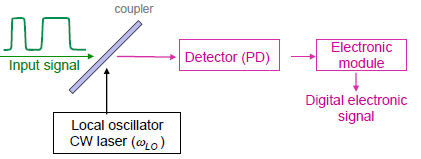
\includegraphics[scale=0.45]{ch6/image37}
	\captionof{figure}{ }
	\end{wrapfigure}
L'objectif principal est de réaliser un récepteur \textbf{limité par le shot noise} en mesurant
à la fois l'amplitude et la phase du signal. Le princise se base sur la génération 
d'\textbf{interférences} entre le signal reçu et une onde continue (\textbf{oscillateur local}) 
\textbf{avant} la détection par une photodiode. \\


Soit le champ électrique du signal d'entrée et celui de l'oscillateur local
\begin{equation}
{E_s} = {A_s}\exp \left( {j[{\omega _s}t + {\phi _s}]} \right),\qquad\qquad
{E_{LO}} = {A_{LO}}\exp \left( {j[{\omega _{LO}}t + {\phi _{LO}}]} \right)
\end{equation}
Quelle est la puissance qui atteint le détecteur ? Faisons l'hypothèse que ces deux champs
ont le même état de polarisation. La puissance reçue est donnée par
\begin{equation}
{P_{in}} = C{\left| {{E_s} + {E_{LO}}} \right|^2} = {P_s} + {P_{LO}} + 2\sqrt {{P_s}{P_{LO}}} \cos \left( {({\omega _s} - {\omega _{LO}})t + {\phi _s} - {\phi _{LO}}} \right)
\end{equation}
Définissons la \textbf{fréquence intermédiaire} $\nu_{if}$
\begin{equation}
{\nu _{if}} = \frac{{|{\omega _s} - {\omega _{LO}}|}}{{2\pi }}
\end{equation}
Si $\nu_{if}=0$, on parle de réception \textbf{homodyne}. Si non, la réception est dite
\textbf{hétérodyne}.

\subsubsection{Homodyne reception ($\omega_{LO}=\omega_s$)}
Soit une podulation OOK, un photodétecteur PIN et un blocage de phase $\phi_{LO}=\phi_s$. Dans ce
cas, la puissance incidente dans le détecteur (PIN) vaut
\begin{equation}
{P_{in}}(t) = {P_s}(t) + {P_{LO}} + 2\sqrt {{P_s}(t){P_{LO}}} 
\end{equation}
Supposons que $P_{LO}\gg P_s$, le terme utile est $2\sqrt {{P_s}{P_{LO}}}$. Nous allons voir que
ceci permet de faire sortir le bruit homodyne du bruit thermique. On appelle le
\textbf{signal homodyne}
\begin{equation}
{I_h}(t) = 2R\sqrt {{P_s}(t){P_{LO}}} 
\end{equation}
Faisons la comparaison avec une détection directe en faisant le rapport entre la puissance en
détection homodyne et le signal reçu directement par le détecteur PIN
\begin{equation}
\frac{{I_h^2}}{{{I^2}}} = \frac{{4{R^2}{P_s}(t){P_{LO}}}}{{{R^2}P_s^2(t)}} = \frac{{4{P_{LO}}}}{{{P_s}}} \gg 1
\end{equation}
Ceci montre que la détection homodyne \textbf{augmente la puissance utile} pour le circuit de
décision \textbf{mais} il augmente le shot noise ($I_h\gg I$).\\

Pour en savoir plus, évaluons le SNR$_e$
\begin{equation}
SN{R_e} = \frac{{{I_h}^2}}{{{\sigma ^2}}} = \frac{{4{R^2}{P_s}{P_{LO}}}}{{\sigma _S^2 + \sigma _T^2}}
\end{equation}
où l'on supposera que le bruit est dominé par le shot noise, rendant $\sigma_T^2$ négligeable. 
En faisant les hypothèses que $P_{LO}\gg P_S$ et $RP_{LO}\gg I_{dark}$, la variance du shot noise
s'écrit
\begin{equation}
 \Rightarrow \sigma _S^2 = 2q\Delta f(R[{P_{LO}} + {P_S} + 2\sqrt {{P_{LO}}{P_S}} ] + {I_{dark}}) \approx 2qR{P_{LO}}\Delta f
\end{equation}
Le SNR$_e$ devient alors
\begin{equation}
SN{R_e} = \frac{{4{R^2}{P_s}{P_{LO}}}}{{2qR{P_{LO}}\Delta f}} = 2\frac{{R{P_s}}}{{q\Delta f}} = 2\eta \frac{{{P_s}}}{{h\nu \Delta f}} \approx \frac{{2\eta }}{{h\nu }}\frac{{N_p^{bit}h\nu 2\Delta f}}{{\Delta f}} = 4\eta N_p^{bit}
\end{equation}
Ce résultat est quatre fois plus élevé que dans le cas d'une détection directe dominée par le
shoit noise ($SN{R^{Shot{\rm{ }}noise}} \approx \eta N_p^{bit}$).\\

Dans la détection homodyne, on peut faire en sorte que le SNR est limité par le shot noise même
si le bruit thermique n'est pas négligeable à condition que
\begin{equation}
\sigma _S^2 = 2qR{P_{LO}}\Delta f \gg \sigma _T^2 = \frac{{4{k_B}T}}{{{R_L}}}{F_n}\Delta f
\qquad\Leftrightarrow\qquad  {P_{LO}} \gg \frac{{\sigma _T^2}}{{2qR\Delta f}} = \frac{{2{k_b}T{F_n}}}{{{R_L}qR}}
\end{equation}
Cette condition sur $P_{LO}$ (de l'ordre de 50 $\mu$W) est très facile à atteindre.\\

Qu'en est-il de la sensibilité du détecteur $\bar{P}_{rec}(Q)$ ? Faisons l'hypothèse que nous
utilisons le seuil de décision optimal, format NRZ, $P_0=0$, que le shot noise domine le bruit
d'intensité et thermique, que $P_{LO}\gg P_1$ et que le bruit d'intensité de l'oscillateur local
n'est \textbf{pas} négligeable ($\sigma_{i,LO}$). Reprenons le courant homodyne
\begin{equation}
{I_1} = R\left( {{P_1} + {P_{LO}} + 2\sqrt {{P_1}{P_{LO}}} } \right),\qquad\qquad
{I_0} = R{P_{LO}},\qquad\qquad
{\bar P_{rec}} = {P_1}/2{\rm{ }}
\end{equation}
On en tire
\begin{equation}
Q = \frac{{{I_1} - {I_0}}}{{{\sigma _1} + {\sigma _0}}} = \frac{{R\left( {{P_1} + {P_{LO}} + 2\sqrt {{P_1}{P_{LO}}} } \right) - R{P_{LO}}}}{{2\sqrt {2qR{P_{LO}}\Delta f + \sigma _{l,LO}^2} }}
\end{equation}
Sachant que ${\sigma _{l,LO}} = RP_{LO}^{}r_{I,LO}^{}$, $Q \approx \frac{{R\sqrt {2{{\bar P}
_{{\rm{rec}}}}{P_{LO}}} }}{{\sqrt {2qR{P_{LO}}\Delta f + {R^2}P_{LO}^2r_{I,LO}^2} }}$, ou encore
\begin{equation}
Q = \sqrt {\frac{{2{{\bar P}_{{\rm{rec}}}}}}{{2q\Delta f{R^{ - 1}} + {P_{LO}}r_{I,LO}^2}}} 
\end{equation}
En en tire la puissance moyenne au récepteur
\begin{equation}
{\bar P_{{\rm{rec}}}} = \frac{{{Q^2}}}{2}\left( {2q\Delta f{R^{ - 1}} + {P_{LO}}r_{I,LO}^2} \right)
\end{equation}
Cette expression montre l'importance du SNR ($=1/r_{I,LO}$) de l'oscillateur local. Si le shot noise
de l'oscillateur local\footnote{Vérifier} domine (c'est-à-dire qu'il est plus important que le bruit
en intensité (de l'oscillateur local))
\begin{equation}
{\bar P_{{\rm{rec}}}} = \frac{{{Q^2}}}{R}q\Delta f = {Q^2}\frac{{h\nu }}{\eta }\Delta f
\end{equation}
Ceci est à comparer avec la détection directe qui donne $\overline {{P_{rec}}}  = \frac{Q}{R}
\left( {Qq\Delta f + {\sigma _T}} \right)$. La sensibilité atteint la limite du shot noise même
pour les récepteurs PIN dont les performances sont limitées par le bruit thermique.\\

Tout a l'air bien, mais nous avons négligé pas mal de choses (NL, Raman, \dots). Il y a deux 
désavantages majeurs à la détection homodyne
\begin{enumerate}
\item Il faut la même fréquence entre le laser maître et l'esclave (mais parfois 400km entre les
deux)
\item La différence de phase $\Delta \phi = \phi_s - \phi_{LO}$ doit rester constante
($I_h\propto \cos(\Delta \phi))$.
\end{enumerate}
Il faut faire une rétroaction sur la phase, ce qui est loin d'être trivial.

\subsubsection{Heterodyne detection ($\omega_{LO}\neq\omega_s$)}
La détection hétérodyne est plus simple à mettre en place. La contrainte sur $\omega_s$ est plus
faible et on peut utiliser $\omega_{LO}$ pour plusieurs canaux. La contrainte sur la stabilité
de la longueur d'onde est également plus faible et il n'y a pas besoin de boucle pour bloquer
la phase. \\

Supposons $P_{LO}\gg P_s$ et
\begin{equation}
{P_{in}} = {P_s}(t) + {P_{LO}} + 2\sqrt {{P_s}(t){P_{LO}}} \cos \left( {({\omega _s} - {\omega _{LO}})t + {\phi _s} - {\phi _{LO}}} \right)
\end{equation}
Il en résulte un signal à la fréquence intermédiaire $\nu_{fi} = (\omega_{LO}-\omega_s)/2\pi$ 
dans les micro-ondes ($\approx 1GHz$). En filtrant pour n'avoir que ce signal (filtre continu)
\begin{equation}
{I_{AC}} = 2R\sqrt {{P_s}(t){P_{LO}}} \cos \left( {2\pi {\nu _{fi}}t + {\phi _s} - {\phi _{LO}}} \right)
\end{equation}
Ce qui correspond à une puissance de signal hétérodyne de $\left\langle {I_{AC}^2} \right\rangle 
 = 2{R^2}{P_s}(t){P_{LO}}$.\\
 
Comparons cette puissance au cas homodyne
\begin{equation}
\frac{{\left\langle {I_{AC}^2} \right\rangle }}{{{I^2}}} = \frac{{2{R^2}{P_s}(t){P_{LO}}}}{{{R^2}P_S^2}} = \frac{1}{2}\frac{{4{P_{LO}}}}{{{P_s}}}
\end{equation}
De par la nature alternative du signal hétérodyne, on perd la moitié de la valeur maximale du signal
obtenue en homodyne, soit une pénalité de 3dB. Avec les mêms hypothèses que pour la détection
homodyne, on trouve
\begin{equation}
SN{R_e} = 2\eta N_p^{bit},\qquad\qquad {\bar P_{{\rm{rec}}}} = 2\frac{{{Q^2}}}{R}q\Delta f
\end{equation}
Ce qui correspond également à une pénalité de 3 dB (prix à payer pour ne pas devoir faire du
phase-locked).


\subsection{Advanced modulation formats}
\subsubsection{1. Amplitude modulation}
On peut faire du On-Off keying (OOK), par exemple en utilisant un Mach-Zehnder pour faire les
interférences destructives.

\begin{center}
	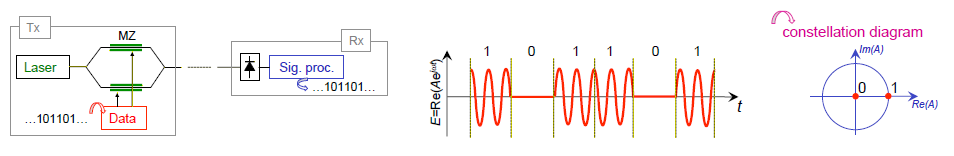
\includegraphics[scale=0.65]{ch6/image38}
	\captionof{figure}{ }
\end{center}

\subsubsection{2. Phase modulation}
\textsc{Binary Phase-shift Keying (BPSK)}\\
A la place d'encoder des niveaux d'amplitude, on va faire des sauts de phase de $\pi$ lorsque
l'on veut envoyer quelque chose. Le modulateur est le même, mais on va appliquer ici la même
tension aux deux bras du MachZehnder (${A_{out}} = {A_{in}}{e^{j\varphi (V)}}$).
\begin{center}
	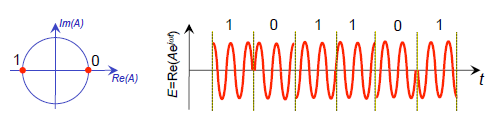
\includegraphics[scale=0.65]{ch6/image39}
	\captionof{figure}{ }
\end{center}
\newpage
Pour le récepteur, c'est moins drôle. Soit le champ électrique du signal ${E_s} = \sqrt {{P_s}} {{\mathop{\rm e}\nolimits} ^{j({\omega _s}t + {\phi _s})}} = {A_s}{{\mathop{\rm e}\nolimits} ^{j{\omega _s}t}}$ et celui de l'oscillateur local ${E_{LO}} = \sqrt {{P_{LO}}} {{\mathop{\rm e}\nolimits} ^{j[{\omega _{LO}}t + {\phi _{LO}}]}}$.
\begin{center}
	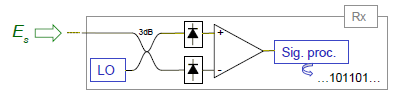
\includegraphics[scale=0.65]{ch6/image40}
	\captionof{figure}{ }
\end{center}


 La puissance reçue est
\begin{equation}
{P_ \pm } = \frac{1}{2}\left( {{P_s} + {P_{LO}} \pm 2\sqrt {{P_s}{P_{Lo}}} \sin [({\omega _s} - {\omega _{LO}})t + {\phi _s} - {\phi _{LO}}]} \right) = \frac{1}{2}\left( {{P_s} + {P_{LO}} \pm 2\sqrt {{P_s}{P_{Lo}}} \cos ({\omega _{IF}}t + \phi )} \right)
\end{equation}
où nous avons utilisé ${\omega _{IF}} = {\omega _s} - {\omega _{LO}}$ et 
$\phi  = {\phi _s} - {\phi _{LO}} - \pi /2$. En faisant la différence entre les deux photo-courants
\begin{equation}
I = R\left( {{P_ + } - {P_ - }} \right) = 2R\sqrt {{P_s}{P_{Lo}}} \cos ({\omega _{IF}}t + \phi )
\end{equation}
On veut retrouver la phase, ce qui gène c'est le $\omega_{if}$. Pour ça, nous allons travailler
dans le domaine électronique
\begin{enumerate}
\item On va retrouver la porteuse dans le microonde $\omega_{if}$
\item On va multiplier ce signal par un signal à cette porteuse généré synthétiquement 
$\cos(\omega_{IF}t)$. Le signal sera alors $\propto \left[ {\cos (2{\omega _{IF}}t + \phi ) + \cos (\phi )} \right]$. 
\item En appliquant un filtre passe-bas, on récupère $R\sqrt {{P_s}{P_{Lo}}} \cos (\phi ) \propto {\mathop{\rm Re}\nolimits} ({A_s})$
\end{enumerate}
Cette méthode requiert une stabilisation de la phase de l'oscillateur local ou un algorithme
pour trouver $\phi_s$.\\



On peut aussi concevoir un récepteur sans oscillateur local. On va mélanger le signal avec
une version retardée de lui même d'exactement un temps symbole $T_S$. Il s'agit d'une méthode
de détection directe : on perd l'augmentation de sensibilité (venant des interférences avec
l'oscillateur local).
\begin{center}
	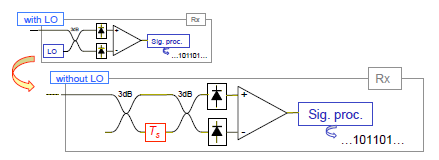
\includegraphics[scale=0.65]{ch6/image41}
	\captionof{figure}{ }
\end{center}
\begin{equation}
{P_ + } = \frac{1}{4}{E_s}(t) + {j^2}{E_s}(t - {T_s}){^2}
\end{equation}
Et donc
\begin{equation}
P_\pm = \frac{1}{4}\left( {{P_s}(t) + {P_s}(t - {T_s})\; \pm [ - {A_s}(t)A_s^*(t - {T_s}) + c.c]} \right)
\end{equation}
Le courant reçu vaut alors (voir calculs \textit{slide 99})
\begin{equation}
{I_{DPSK}} = R({P_ - } - {P_ + }) = \frac{R}{2}\left( {[{A_s}(t)A_s^*(t - {T_s}) + c.c]} \right) = R{\mathop{\rm Re}\nolimits} \left( {{A_s}(t)A_s^*(t - {T_s})} \right)
 = R{P_s}\cos (\Delta \phi )
\end{equation}
On peut alors retrouver le signal d'entrée par un traitement des données (mais il faut encoder
les donnée dans la différence de phase entre deux bits adjacents\footnote{Expliciter.}).\\


\textsc{Differential BPSK (DBPSK)}\\
On effectue un saut de phase seulement lorsque l'on veut coder un zéro. Il faut que la phase du 
laser soit stable sur au moins 2 bits.
\begin{center}
	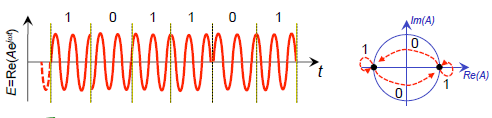
\includegraphics[scale=0.65]{ch6/image42}
	\captionof{figure}{ }
\end{center}
Les méthodes BPSK et DBPSK n'augmentent pas l'efficacité comparé au OOK, mais le format de modulation
permet d'encoder plus de bits sur un symbole et augmenter l'efficacité spectrale.\\

\textsc{Quadrature PSK (QPSK) or Differential QPSK (DQPSK)}\\
Il s'agit d'une modulation purement en phase, mais à la place d'avoir des sauts de phase de 0 et
$\pi$, on aura également $\pi/2$ et $3\pi/2$. Ceci permet d'avoir un débit binaire valant deux fois
le débit symbole mais le modulateur est plus compliqué (besoin d'une partie réelle et imaginaire). 
On utilise un MZ dédoublé. 
\begin{center}
	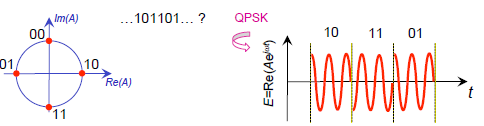
\includegraphics[scale=0.65]{ch6/image43}
	\captionof{figure}{ }
\end{center}
Pour le \textbf{récepteur, voir \textit{slide 102}}\footnote{QR !!}\\
\begin{center}
	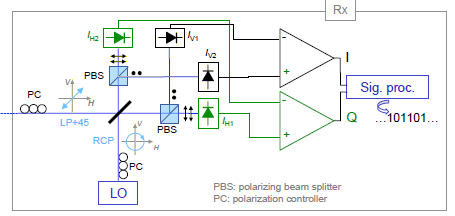
\includegraphics[scale=0.65]{ch6/image44}
	\captionof{figure}{ }
\end{center}

\textsc{Phase shift keying (PSK) \& quadrature amplitude modulation (QAM)}\\
On peut faire mieux que quatre points sur la constellation. En modulant en amplitude et en phase,
on peut faire n'importe quelle constellation. Un format de modulation plus rapide que le binaire
permet de réduire le taux de symbole et ainsi limiter les impacts de la propagation (dispersion
chromatique, PMD). Hélas, cela rend le système plus sensible au bruit.
\begin{center}
	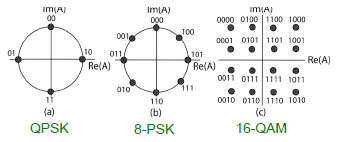
\includegraphics[scale=0.65]{ch6/image45}
	\captionof{figure}{ }
\end{center}



\textsc{Polarization multiplexing QPSK (PM-QPSK)}\\
En exploitant l'état de polarisation de la porteuse optique, l'efficacité spectrale peut être encore augmentée par un facteur de deux: Deux flux binaires sont envoyés simultanément à la même longueur d'onde mais sur deux états de polarisation orthogonaux. Le \textit{slide 105} donne un exemple
de transmetteur. Voir aussi \textit{slide 106}.
\begin{center}
	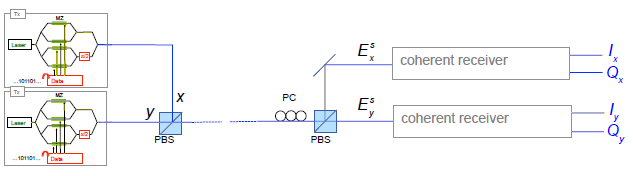
\includegraphics[scale=0.65]{ch6/image46}
	\captionof{figure}{ }
\end{center}



\subsection{Electronic compensation of propagation impairments}
Dans les détecteurs cohérent, on mesure l'amplitude et la phase. Mais avant de passer dans le
circuit de décision, un signal digitalisé peut être traité pour compenser les différentes 
distorsions. 

\subsubsection{Chromatic dispersion compensation}
\begin{wrapfigure}[10]{l}{7cm}
	\vspace{-5mm}
	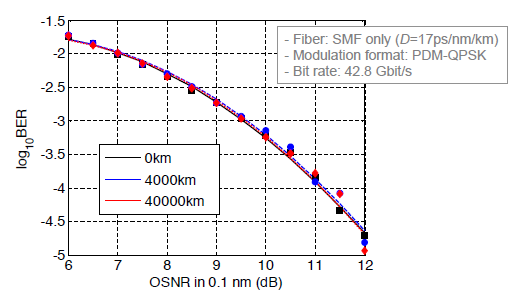
\includegraphics[scale=0.45]{ch6/image47}
	\captionof{figure}{ }
	\end{wrapfigure}
Dans un régime linéaire, la fibre optique est un système linéaire dont la fonction de 
transfert est donnée par
\begin{equation}
\tilde H(\omega ) = \exp ( - j\int\limits_0^L {\beta (\omega ,z)dz} )
\end{equation}
On peut compenser la dispersion chromatique dans le domaine temporel\\
\\

\begin{enumerate}
\item Prendre la TF du signal digitalisé
\item Multiplier la TF par l'inverse de la fonction de transfert
\begin{equation}
{\tilde H^*}(\omega ) = \exp ( + j\int\limits_0^L {\beta (\omega ,z)dz} )
\end{equation}
\item Prendre la TF inverse du résultat
\end{enumerate}

Ceci permet de compenser en une fois toute la dispersion dans le détecteur sans avoir 
besoin d'utiliser des DCF avec plein de non-linéarité. Comme le régime est linéaire, tout
est préductible. Il n'y a donc pas de pénalité ici!

\subsubsection{PMD compensation}
Lorsque le récepteur enregistre les deux polarisations, on peut compenser la PMD en utilisant
l'inverse de la matrice de Jones estimée. On peut écrire des algorithmes qui construisent la
matrice de Jones des données reçue en fonction du format de modulation. Le système de compensation
 doit être adaptatif car la PMD dépendant du temps.


\section{Conclusion and outlook}
\begin{center}
	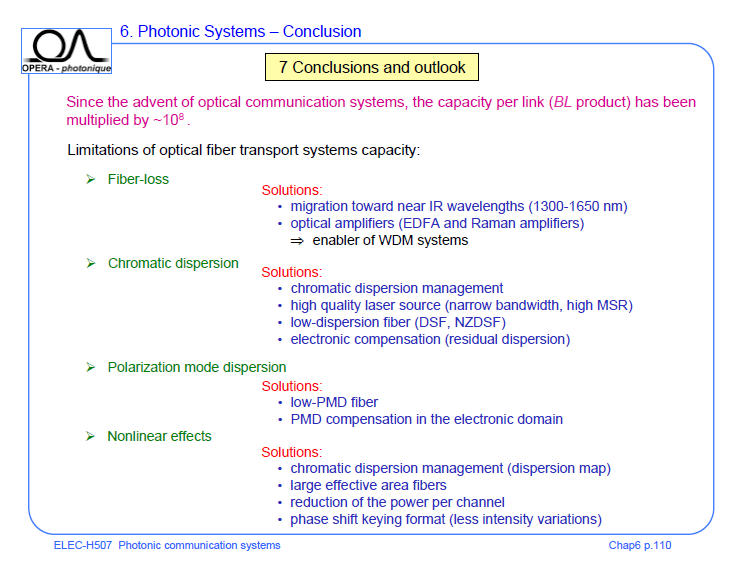
\includegraphics[scale=0.55]{ch6/image48}
%	\captionof{figure}{ }
\end{center}


\begin{center}
	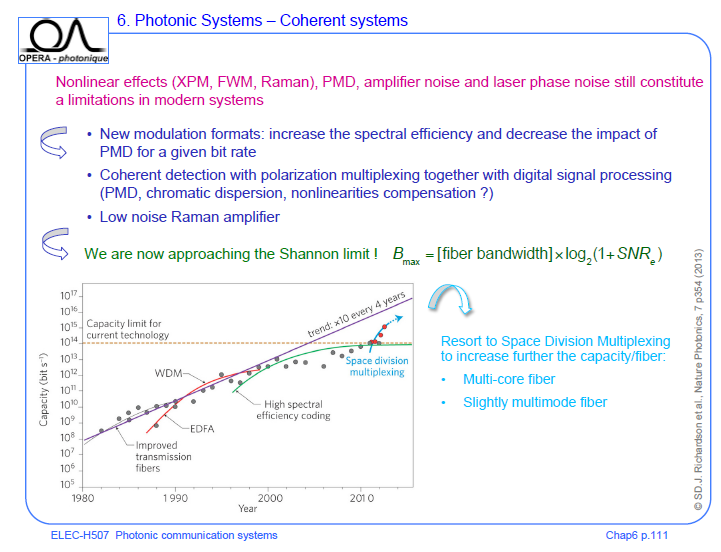
\includegraphics[scale=0.55]{ch6/image49}
%	\captionof{figure}{ }
\end{center}



